\chapter{Simulations}
The numerical simulations studied in this section define the main tool for evaluation and validation of the ultrasound technique. It includes assessment of the homogenized coefficient predictions by means of the FEM method under the clinical-range of porosities with regards to standard literature, elastodynamic simulations associated to the experimental device on time-and frequency formulations described in the section before and the processing of \textit{Lamb}-modes characterizing the material behavior recorded at the receivers. In this context, aspects such as computational costs, fidelity derived from the meshes and instabilities are faced at various degrees of success.
Moreover, \texttt{Python} source code to recreate the results is freely available at the repository \href{www.github.com/PublicMistakes/Codes}{Codes}.

\section{Numerical Solutions to Cell Problems}
Following the developments done before to obtain effective equations governing the macroscopic mechanical behavior of cortical bone, one of the main difficulties to solve is related to the so-called cell problems which contains the non-linear component associated to the homogenized coefficients.
Such a PDE problem is characterized by unique vector-valued solutions $\mathbf{N}^{rs} \in \mathbf{H}^1_{\#} (\mathbf{Y})$ for each $r,s \in \{1,\dots, d\}$ satisfying the elliptic PDE system:
\begin{equation*}
    \label{CellProblem-System}
    \left \{
    \begin{array}{cc}
        - \partial_{y_j} \big[C_{ijkl}(\mathbf{y}) \mathbf{e}_{kl,y} \big( \mathbf{N}^{rs}(\mathbf{y}) \big)  \big] = \partial_{y_j} \big( C_{ijrs} (\mathbf{y}) \big)& \text{ in } \mathbf{Y} \\
        \big[ C_{ijkl}(\mathbf{y}) \mathbf{e}_{kl,\mathbf{y}}\big( N^{rs}(\mathbf{y}) \big) \big]n_j = 0 &  \forall \mathbf{y} \in \partial Y
    \end{array}
    \right.
\end{equation*}
where its added the condition 
\begin{equation*}
    \int_{\partial Y} N^{rs}(\mathbf{y}) \, d\mathbf{y} = \mathbf{0}
\end{equation*}
to obtain uniqueness, since the right hand side to \ref{CellProblem-System}) is constructed satisfies average equal to $\mathbf{0}$.
The variational formulation is then given by integration by parts, where for $\phi \in \mathbf{H}^1_{\#}(\mathbf{Y})$ it follows:
\begin{equation*}
    \int_{Y} C_{ijkl}(\mathbf{y}) \mathbf{e}_{kl,\mathbf{y}}(N^{rs}(\mathbf{y})) \partial_{y_j}\phi_i = - \int_{Y}C_{ijrs}(\mathbf{y}) \partial_{y_j} \phi_i + \int_{\partial Y}C_{ijrs}(\mathbf{y}) n_j \phi_i
\end{equation*}

Considering the standard biomechanical literature, the bone matrix is mainly made from hydroxyapatite, a material which can be modeled with a linear elastic behavior and inclusion defining the mesoscale composed mainly of saturated fluid, described with viscoelastic type behavior which in this approximation it is considered of static elastic material. Taking axial symmetry along the long axis of bone, the composed material is modeled with transverse isotropy in each component $C^m_{ijkl}$, $C^f_{ijkl}$ of matrix and water phases respectively.
It follows then the elastic tensors $C_{ijkl}$ defined on the cell $\mathbf{Y}$ by
\begin{equation*}
    C_{ijkl} (\mathbf{y}) := C^m_{ijkl} \mathbb{I}_{\{\mathbf{y} \in  \mathbf{Y}_{m}\}} + C^f_{ijkl} \mathbb{I}_{\{ \mathbf{y} \in \mathbf{Y}_{p}\}}
\end{equation*}
Such isotropic elastic behavior can be described explicitly using \textit{Voigt} notation as a $6\times 6$ matrix in the 3-dimensional case by:
\begin{equation*}
    C_{ij}(\mathbf{y}) = 
    \begin{bmatrix}
    C_{11}(\mathbf{y}) & C_{12}(\mathbf{y}) & C_{13}(\mathbf{y}) & 0 & 0 & 0 \\
    C_{12}(\mathbf{y}) & C_{11}(\mathbf{y}) & C_{23}(\mathbf{y}) & 0 & 0 & 0 \\
    C_{13}(\mathbf{y}) & C_{23}(\mathbf{y}) & C_{23}(\mathbf{y}) & 0 & 0 & 0 \\
    0 & 0 & 0 & C_{44}(\mathbf{y}) & 0 & 0 \\
    0 & 0 & 0 & 0 & C_{44}(\mathbf{y}) & 0 \\
    0 & 0 & 0 & 0 & 0 & C_{66}(\mathbf{y}) 
    \end{bmatrix}
\end{equation*}

which is given by the transverse isotropy symmetries of the material components. In particular, it is assumed that $C_{55}(\mathbf{y}) = C_{44}(\mathbf{y})$ and $C_{11}(\mathbf{y}) = C_{22}(\mathbf{y})$.

Simulations are done of the homogenized coefficients in function of the porosity level, i.e. setting the circular inclusion with radius $r(p)$ being $p \in (0,1)$ the set of admissible porosity levels, in the form $ p := \frac{\vert \mathbf{Y}_f \vert }{\vert \mathbf{Y}\vert} $. Moreover, 2-dimensional and 3-dimensional cases are assumed over the micrsotructure to assess different aspects of symmetry.

Explicitly, an increasing array of possible porosity levels is chosen limited to the value-ranges of interest, i.e. it's limited to the $[0, 0.3]$ interval of possible porosities. The numerical solution to the model is obtained using the \texttt{UFL} language implemented within the library \texttt{FEniCS}\footnote{The \texttt{FEniCS} project \cite{logg2012automated} is an international initiative, started in 2013 with the objective to automate the solution of mathematical models based of Partial Differential Equations of the type elliptic as the heat equation, hyperbolic as the wave equation, quasi-hyperbolic equations, etc., using the Finite Element theory and formalism to find such solution. More in general, its capable to find an approximate solution by means of a well-posed general variational formulation. Different use scenarios can be seen at \cite{abali2016computational}.\\
Defined as a set of interdependent base \texttt{C++} libraries such as \texttt{DOLFIN} \cite{LoggWells2010a}, \texttt{FIAT}, \texttt{SFC} to just mention some. \texttt{FEniCS} implements a close-to-abstract coding and procedure to solve PDE problems on interface languages such as the native \texttt{C++} or via wrappers \texttt{Python}. Moreover, such base libraries rely on high-performance libraries for the algebra computations necessary in the FEM, such as \texttt{PETSc} which implements iterative solver of \textit{Krylov} type and a range of preconditioner to find an approximate solution $x \in \mathbb{R}^m$ of $Ax = b$ for $\mathcal{M}_{m \times m}(\mathbb{R})$, $b \in \mathbb{R}^m$ for $m \gg 1$.} to solve PDE's in variational formulation. In particular, it is used the \texttt{PETScKrylov} solver to solve the matrix system obtained after discretize the variational formulation by FEM, and over such solver we used the \texttt{GMRES} (Generalized Minimal Residual Method)\footnote{The \texttt{GMRES} method is an efficient algorithm to solve large linear systems. It uses an iterative method associated to the Theory of Krylov subspaces to approximate the solution of the system by reducing the high dimensional problem to a sequence of low dimensional, solved each one by least squares.
Explicitly, given $A \in \mathcal{M}_{m\times m} (\mathbb{R})$, $b \in \mathbb{R}^m$ for $m\gg 1$, the \texttt{GMRES} algorithm solves the problem $A x = b$ by solving the problems 
\begin{equation*}
    \underset{x \in \mathcal{K}_n}{\text{ min }} \Vert b - Ax \Vert_2   
\end{equation*} 
for increasing values of $n \in \mathbb{N}$, knowing $\mathcal{K}_n = \mathcal{K}_n(A,b)$ the Krylov space of order $n$ defined by
\begin{equation*}
 \mathcal{K}_n(A,b) = \text{span }\{ b, Ab, \dots, A^{n-1}b \} \subset \mathbb{R}^m   
\end{equation*}
At each iteration, its computed the residual by least squares, where under reasonable assumptions of symmetry of the matrix, the residual will be sufficiently small for $n \ll m$.} with preconditioner given by \textit{iLU} (incomplete LU factorization). Such consideration where done to tackle in numerical instabilities and non-convergence results shown, assembling a linear system sparse with better properties for numerical inversion.

The predictions are then compared with the approximation of the homogenized coefficients for cortical bone using the same input coefficient tensor of \textit{Parnell} and \textit{Grimal} (PG), whom by means of a multipolar approximation of the solution to (\ref{CellProblem-System}) obtained semi-analytic approximate expressions for the solution \cite{Parnell2008}, thus enabling in this case a comparison to a FEM method proposed here to solve each of the cell problems involved in the homogenized coefficient description. It's important to emphasize that PG solutions define the standard reference used in literature and a relevant comparison study must be made to test validity and robustness under different configuration.

\subsection{2-Dimensional Models}
Taking into account the symmetry condition assumed for the microstructure described as repetition along the long axis of bone, motivates the consideration of $d = 2$ over a unit square microstructure domain, i.e. $\mathbf{Y} = (0,1)^2$. While the porosity is of circular type.

The figure (\ref{MainHomCoeffsSquare}) contains the predictions of the diagonal homogenized elastic coefficients by means of the FEM, compared to the results obtained from PG. It's shown a close behavior for the results, and moreover in two different mesh sizes. The representative isotropic values in particular, shows differences with a error percentages $< 5 \%$ validating the numerical solutions.
\begin{figure}[!h]
	\centering
	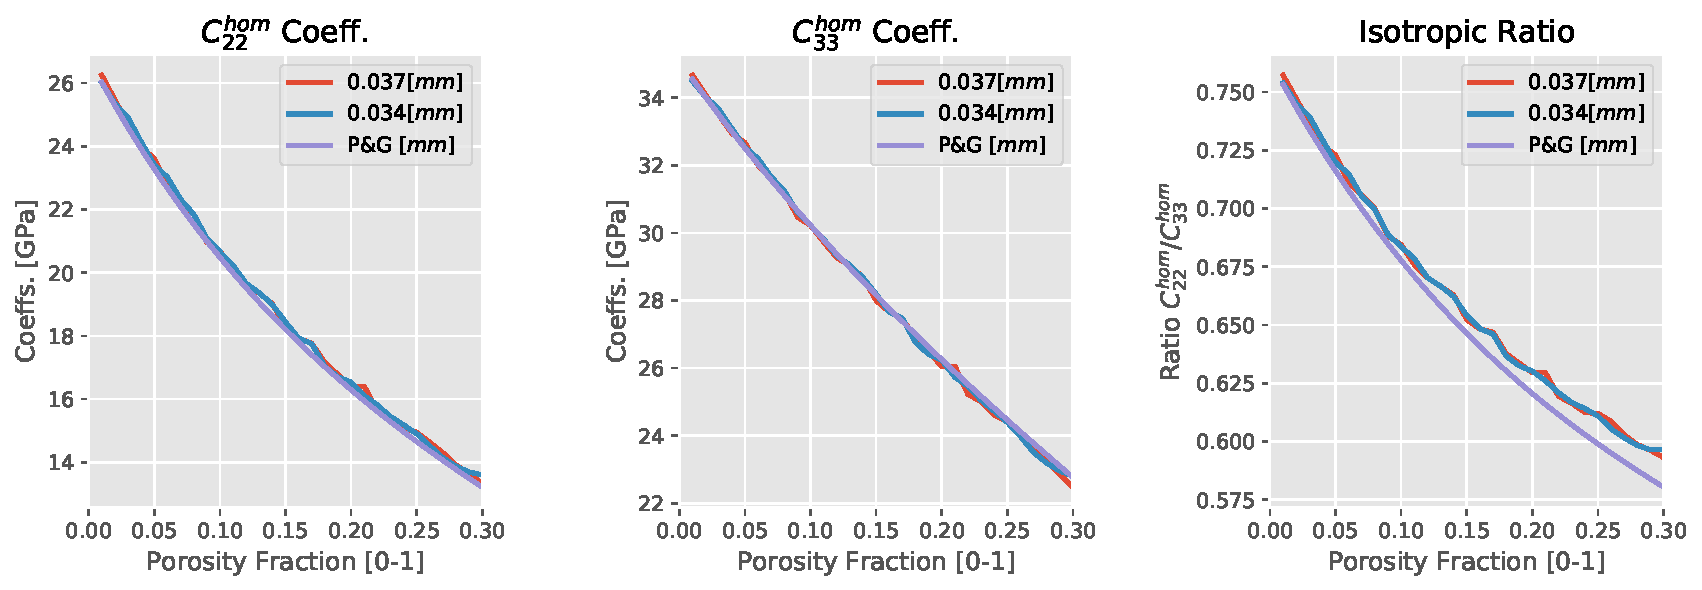
\includegraphics[scale=.5]{images/CellsProb/CellProb_MainHomCoeffsCircular.pdf}
	\caption{Main diagonal elastic homogenized coefficients in \textit{Voigt} notation. They describe an transverse isotropic behavior, spanned in the figure on the biomedical range of $(1,30) [\%]$ cortical porosity. The characteristic microstructure in this case is of unitary square. The blue, orange lines describe the FEM predictions at different mesh sizes, whereas the green line describes the PG approximation.}
	\label{MainHomCoeffsSquare}
\end{figure}
Similarly, figure (\ref{OtherHomCoeffsSquare}) shows the non-diagonal homogenized coefficients that describe the shear behavior again compared to the PG reference case. It shows moreover a lower percentage error in all the coefficients describing the mechanical behavior related to the axial plane (in this case $C_{55}^{hom}, C_{23}^{hom}$), whereas the $C_{66}^{hom}$ that describes full shear interaction on the anti-axial plane, shows a clear difference toward bigger porosity values with $> 5\%$ percentage errors. 
Such failure in the prediction can be attributed to errors regarding to the boundary conditions \textit{Neumann} conditions being imposed, and moreover to the assumption on the characteristic microstructure. Nevertheless, as the PG predictions for the $C_{66}^{hom}$ are validated with respect to experimental data results under an error percentages of $> 5 \%$, the solutions found for such coefficient cannot be rejected since the predictions in are in the same range of error percentages.

\begin{figure}[!h]
	\centering
	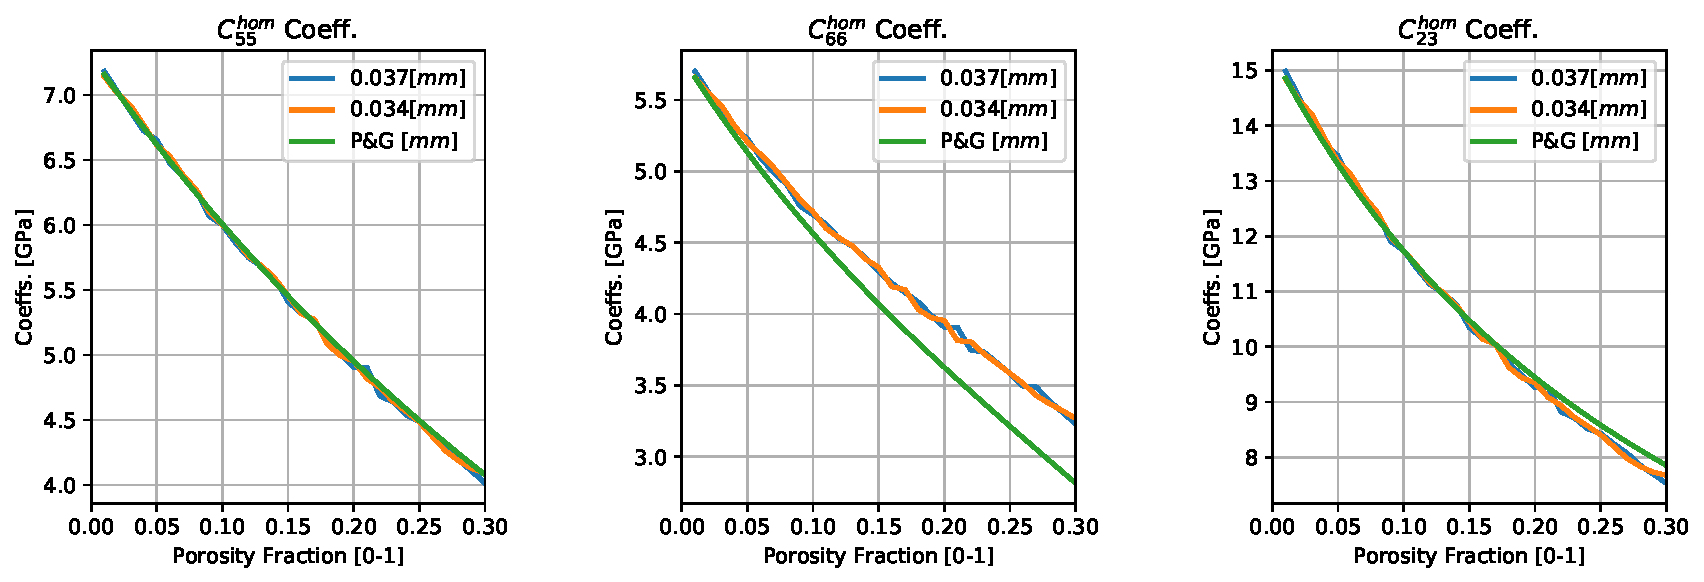
\includegraphics[scale=.5]{images/CellsProb/CellProb_OthersHomCoeffsCircular.pdf}
	\caption{Other diagonal elastic homogenized coefficients in \textit{Voigt} notation. They describe an transverse isotropic behavior, spanned in the figure on the biomedical range of $(1,30) [\%]$ cortical porosity with unitary square characteristic microstructure.}
	\label{OtherHomCoeffsSquare}
\end{figure}

The explicit results of error percentages associated to the predictions for the complete homogenized elastic tensor are shown in table (\ref{HomCoeffSquareTable}). It describes the clear correspondence between coefficients associated to the axial plane with errors $< 0.1\%$, whilst differences over all anti-axial coefficients such as $C_{12}^{hom}, C_{66}^{hom}$.
\begin{table}[!h]
\centering
    \begin{tabular}{ |p{2.2cm}||p{2cm}|p{2cm}|p{2cm}|p{2cm}| }
    \hline
    \multicolumn{5}{|c|}{\textbf{Homogenized Coefficients}} \\
    \hline
    \textbf{Error} [\%] & $\phi = 5 \%$ & $\phi = 10 \%$ & $\phi = 15 \%$ & $\phi = 20 \%$ \\
    \hline
    $C^{hom}_{22}$ & 0.6 \% & 1.3 \% & 1.3 \% & 1.5 \% \\
    $C^{hom}_{33}$ & <0.1 \% & <0.1 \% & <0.1 \% & <0.1 \% \\
    $C^{hom}_{55}$ & <0.1 \% & <0.1 \% & <0.1 \% & <0.1 \% \\
    $C^{hom}_{66}$ & 1.4 \% & 3.3 \% & 6.3 \% & 9.0 \% \\
    $C^{hom}_{12}$ & <0.8 \% & 1.5 \% & 3.3 \% & 5.9 \% \\
    $C^{hom}_{23}$ & 0.4 \% & <0.1 \% & 0.3 \% & 1.0 \% \\
    \hline
    \end{tabular}
    \caption{Percentage errors of the homogenized coefficient with respect to the PG reference case. The tensors are written in \textit{Voigt} notation and microstructure is defined by a 2-dimensional unitary square with periodic perforation as porosity as shown schematically in (\ref{HomBasicScheme}).}
    \label{HomCoeffSquareTable}
\end{table}

To assess the high error percentage obtained from (\ref{HomCoeffSquareTable}) shown on the non-axial related coefficients within the 2-dimensional domain, its proposed to study a hexagonal type domain following the idealization proposed from \cite{Parnell2008}. In this sense, it's expected corrections over the cell-problems that could contribute to such assumption.

In the following, it will be considered a 2-dimensional hexagonal polygon domain with porosity inclusion of circular type. As before, simulations are done using the same solver proposed for the square case, the linear system derived from the governing system (\ref{CellProblem-System}) is solved preconditioned using an iterative solver.

The figure (\ref{MainHomCoeffHexa}) described the predictions results for the diagonal coefficients in this case by the FEM method, compared to the reference results. Its shows a clear prediction on the two main diagonal coefficients, being the isotropic values with percentage errors $< 1 \%$, thus being a best prediction in this cases.
\begin{figure}[!h]
	\centering
	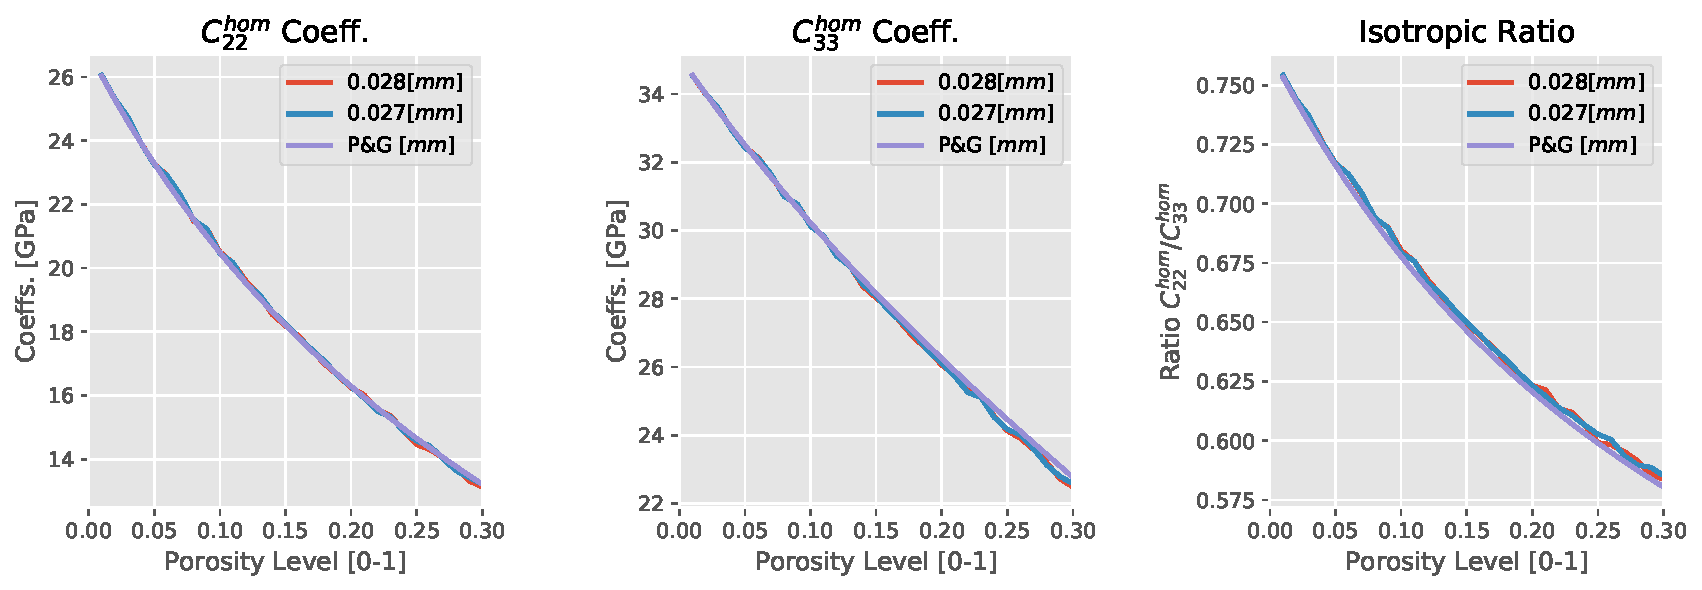
\includegraphics[scale=.5]{images/CellsProb/CellProb_MainHomCoeffsCircularHexa.pdf}
	\caption{Main diagonal elastic tensor coefficients in \textit{Voigt} notation. The figure shows the prediction values over the range $(1,30) [\%]$ of porosities with characteristic microstructure defined by an hexagonal 2-dimensional polygon. The blue, orange lines describe the FEM predictions at different mesh sizes, whereas the green line describes the PG approximation.}
	\label{MainHomCoeffHexa}
\end{figure}
Similarly, figure (\ref{OtherHomoCoeffsHexa}) shows the non-diagonal elastic coefficients describing shear behavior comparing again to (PG) approximations. The coefficients connected to the axial-plane shows predictions with errors $< 2 \%$ thus validated under the clinical range, whereas the problematic prediction on the $C_{66}^{hom}$ coefficient persist as in the case before and moreover, the errors become $> 15 \%$ at bigger porosity values. Again, the prediction failure is assessed to the boundary conditions being imposed on the domain, and the continuity conditions over the mesh. The instability effects obtained, shows a clear dependence on the mesh size, thus further studies must be done.
\begin{figure}[!h]
	\centering
	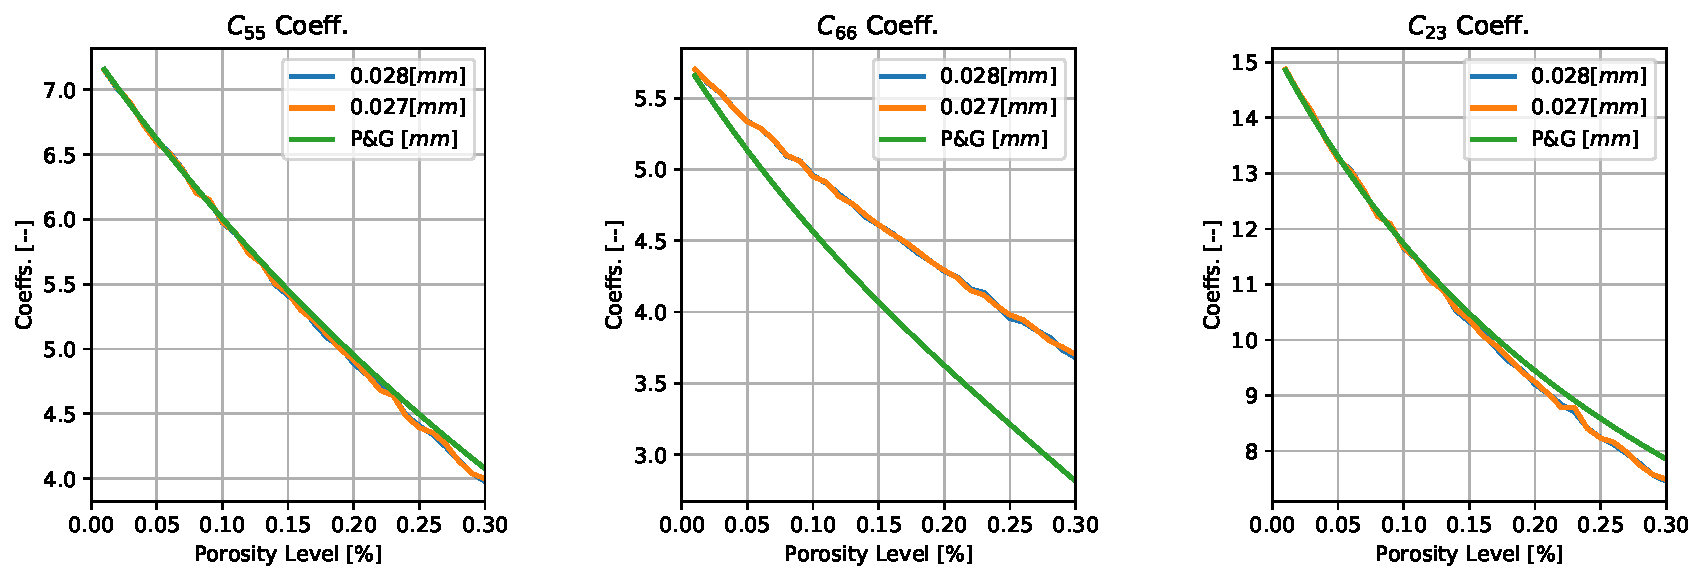
\includegraphics[scale=.5]{images/CellsProb/CellProb_OthersHomCoeffsCircularHexa.pdf}
	\caption{Shear type elastic homogenized coeffs. in \textit{Voigt} notation. The figure shows the behavior over the range $(1,30) [\%]$ porosity with characteristic microstructure described by a hexagonal 2-dimensional polygon.}
	\label{OtherHomoCoeffsHexa}
\end{figure}
Finally, the explicit results of percentage errors are shown in the table (\ref{HomCoeffHexaTable}). It describes the clear correspondence between elastic homogenized coefficients with axial connection, and the error prediction on the $C_{66}^{hom}$ which is attributed to a full non-axial behavior, not captured within the 2-dimensional microstructure assumption.

\begin{table}[!h]

\centering
    \begin{tabular}{ |p{2.2cm}||p{2cm}|p{2cm}|p{2cm}|p{2cm}| }
    \hline
    \multicolumn{5}{|c|}{\textbf{Homogenized Coefficients}} \\
    \hline
    \textbf{Error} [\%] & $\phi = 5 \%$ & $\phi = 10 \%$ & $\phi = 15 \%$ & $\phi = 20 \%$ \\
    \hline
    $C^{hom}_{22}$ & <0.1 \% & <0.1 \% & <0.1 \% & 0.3 \% \\
    $C^{hom}_{33}$ & 0.2 \% & 0.3 \% & 0.1 \% & 0.7 \% \\
    $C^{hom}_{55}$ & 0.3 \% & 0.5 \% & 0.1 \% & 1.2 \% \\
    $C^{hom}_{66}$ & 4.0 \& & 8.6 \% & 13.2 \% & 18.2 \% \\
    $C^{hom}_{12}$ & 0.7 \% & 2.1 \% & 4.4 \% & 7.2 \% \\
    $C^{hom}_{23}$ & 0.2 \% & 0.7 \% & 1.4 \% & 2.5 \% \\
    \hline
    \end{tabular}
    \caption{Percentage errors between the homogenized coefficients and the PG reference case. The tensors are expressed in \textit{Voigt} notation with microstructure defined as a hexagonal polygon with circular perforation acting as porosity.}
    \label{HomCoeffHexaTable}
\end{table}

From tables (\ref{HomCoeffSquareTable}), (\ref{HomCoeffHexaTable}) it can be concluded that the 2-dimensional axial type description of the characteristic periodic microstructure relates correctly to realistic mechanical behavior in bone, nevertheless it lacks of non-axial type description regarding to PG predictions. It related then to a possible failure to incorporate non-axial structures that marginally could affect the homogenized coefficients by means of the two-scale framework. Such effects are currently under study in a experimentally oriented setting \cite{Cai2019}.

\subsection{3-Dimensional Model}
To test the insight observed using 2-dimensional case and assuming the lower percentage error shown from the unit-square type domain, a 3-dimensional cubic domain with cylindrical type inclusion is proposed as periodic microstructure characteristic of cortical bone, i.e. $\mathbf{Y} = (0,1)^3$. Such new degree of freedom is expected to contribute on the non-axial behavior, thus incorporating missing elements that vanish from a lower dimensional description. However, it requires computational cost associated to finer meshes for fidelity results. \\

The figure (\ref{Main3dHomCoeffSquare}) describes diagonal coefficients by means of FEM method, comparing with PG predictions. Nevertheless, the isotropic ratio predicts a different behavior from the 2-dimensional models, assumed from the new terms describing multiple axial and anti-axial interaction on the cell PDE system. 
\begin{figure}[!h]
	\centering
	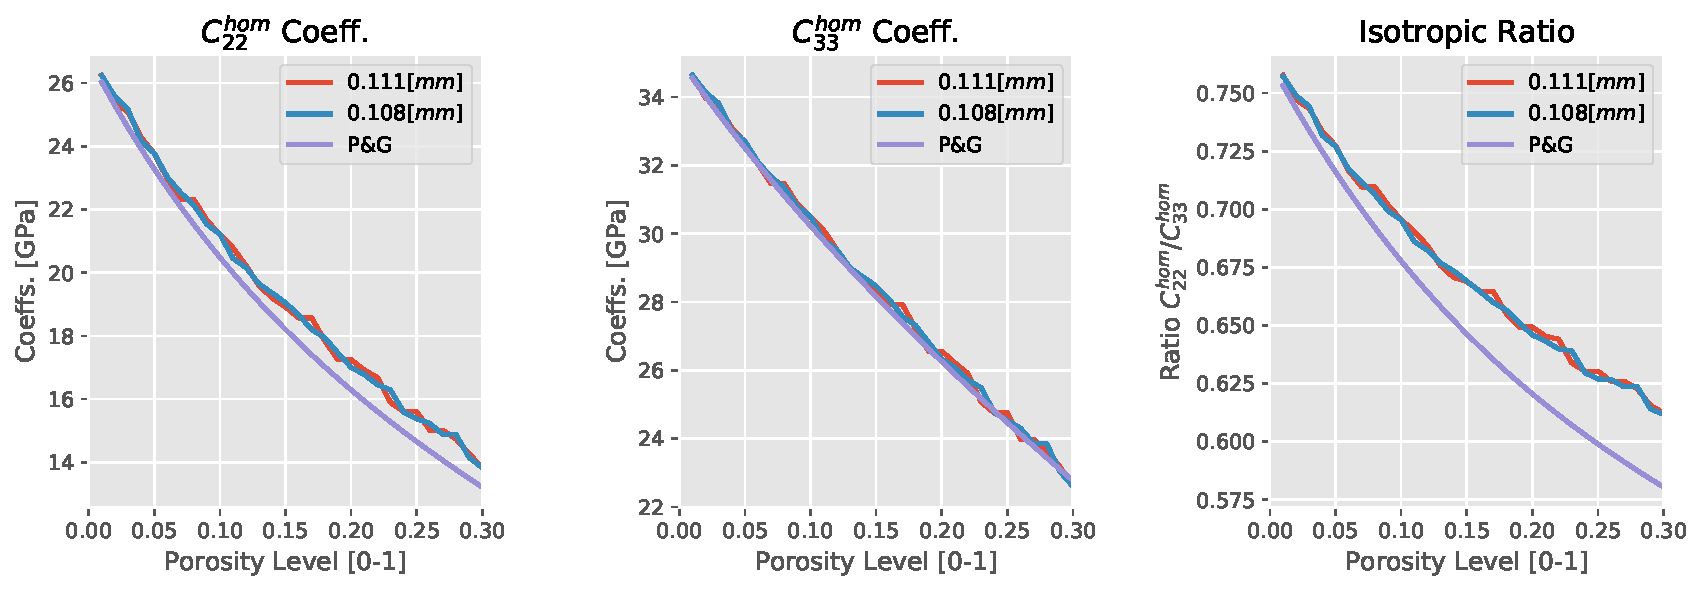
\includegraphics[scale=.5]{images/CellsProb/3DCellProb_MainHomCoeffsCircular.pdf}
	\caption{Main diagonal elastic tensor coefficients in \textit{Voigt} notation. It describes prediction values over the range $(1,30) [\%]$ of porosities with 3-dimensional cubic characteristic microstructure. The blue, orange lines describe the FEM predictions at different mesh sizes, whereas the green line describes the PG approximation.}
	\label{Main3dHomCoeffSquare}
\end{figure}
Similarly, (\ref{Other3dHomCoeffSquare}) describes no-diagonal coefficients that in 2-dimensional case contains the greater error percentages. As stated before, such behavior assumed to be interactions between non-axial and axial behaviors as described from $C_{55}^{hom}, C_{23}^{hom}$ coefficients shows error of $\sim 1 \%$ regarding to PG predictions. Thus, such error percentages result close to 2-dimensional models tested before, but it remains a different behavior on the $C_{66}^{hom}$ coefficient with error $\sim 10 \%$.

\begin{figure}[!h]
	\centering
	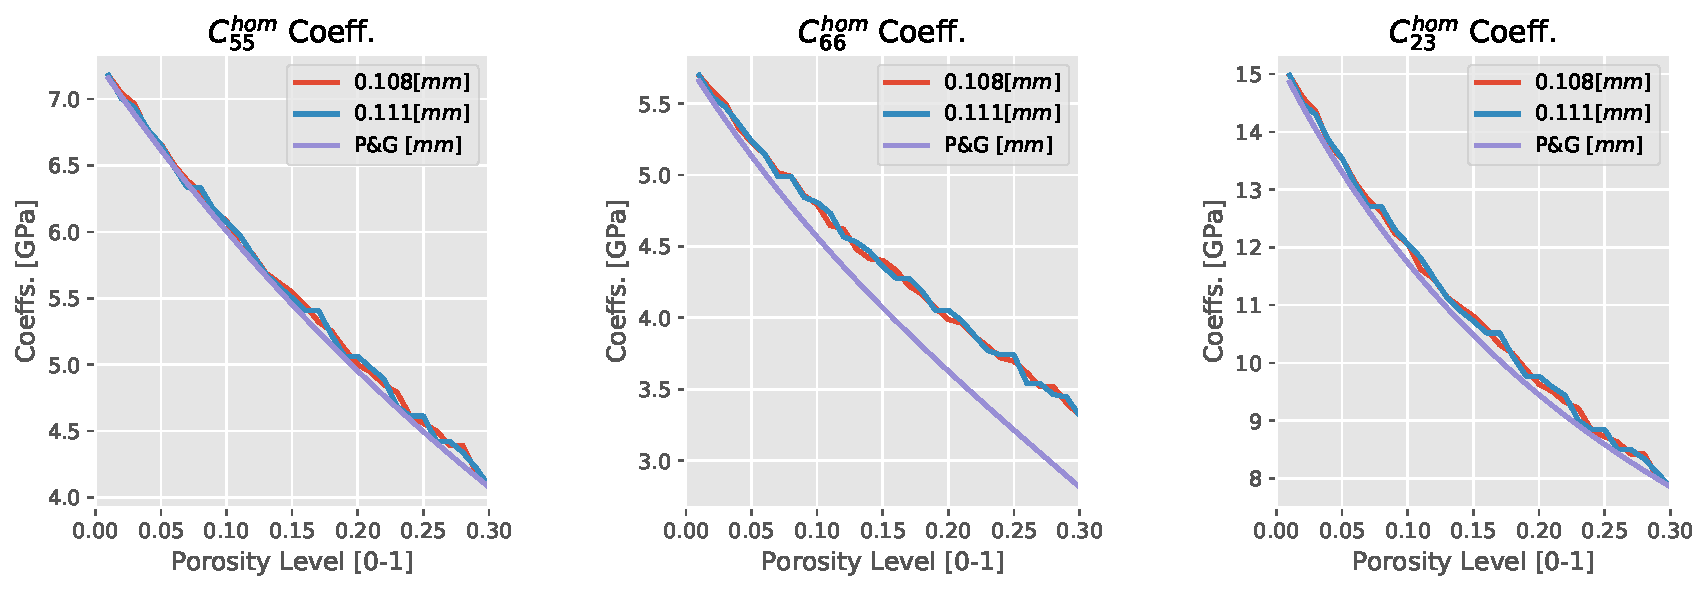
\includegraphics[scale=.5]{images/CellsProb/3DCellProb_OthersHomCoeffsCircular.pdf}
	\caption{Main diagonal elastic tensor coefficients in \textit{Voigt} notation. It describes prediction values over the range $(1,30) [\%]$ of porosities with 3-dimensional cubic characteristic microstructure. The blue, orange lines describe the FEM predictions at different mesh sizes, whereas the green line describes the PG approximation.}
	\label{Other3dHomCoeffSquare}
\end{figure}

Finally, table (\ref{Hom3dCoeffSquareTable}) shows explicitly error percentages obtained at various porosity levels. It can be concluded that, diagonal elastic coefficients describes with lower errors the mechanical behavior following PG asymptotic solutions, as shown by $C_{22}^{hom}, C_{33}^{hom}$. With similar characteristics, axial interacting coefficients such as $C_{23}^{hom}, C_{55}^{hom}$ follows predicted values regarding the reference which implies correct incorporation of realistic interaction within long bone axis. Nevertheless, $C_{66}^{hom}$ remains with higher errors of $\sim 10 \%$ which enable us to conclude possible underlying effects from produced from the microstructure, having impact on the overall elastic behavior on bone. Such conclusion it backed-up from the validity of PG model, which fits experimental data with $C_{66}^{hom}$ errors of $\sim 9 \%$. It can be associated moreover to the presence of \textit{Volksmann} canals that interact on the non-axial plane and that are assumed to have minimal impact on the periodic structure, which might not be fully valid at this scale.

\begin{table}[!h]
\centering
    \begin{tabular}{ |p{2.2cm}||p{2cm}|p{2cm}|p{2cm}|p{2cm}| }
    \hline
    \multicolumn{5}{|c|}{\textbf{Homogenized Coefficients}} \\
    \hline
    \textbf{Error} [\%] & $\phi = 5 \%$ & $\phi = 10 \%$ & $\phi = 15 \%$ & $\phi = 20 \%$ \\
    \hline
    $C^{hom}_{22}$ & 2.1 \% & 3.5 \% & 4.6 \% & 4.3 \% \\
    $C^{hom}_{33}$ & 0.5 \% & 0.9 \% & 1.0 \% & 0.2 \% \\
    $C^{hom}_{55}$ & 0.6 \% & 1.3 \% & 1.6 \% & 0.9 \% \\
    $C^{hom}_{66}$ & 1.8 \% & 5.0 \% & 8.1 \% & 9.9 \% \\
    $C^{hom}_{12}$ & 1.4 \% & 1.7 \% & 0.9 \% & 2.1 \% \\
    $C^{hom}_{23}$ & 1.8 \% & 2.7 \% & 3.1 \% & 1.9 \% \\
    \hline
    \end{tabular}
    \caption{Percentage errors between the homogenized coefficients and the PG reference case. The tensors are expressed in \textit{Voigt} notation with 3-dimensional cubic microstructure and cylindrical subdomain describing the porosity.}
    \label{Hom3dCoeffSquareTable}
\end{table}

\section{2-Dimensional Simulations of Wave Propagation}
The simulation setting associated to the experimental measurements is defined by a 2-dimensional rectangular array imitating the frontal plane associated to the cortical bone. In this case, the wave-propagation can be directly compared to the \textit{Lamb}-wave  theory proposed by \textit{Rhee} in \cite{Rhee2007}, thus enabling the numerical validation of the modelling being used. 

The transducer excitation source is defined at the upper surface where the omit the interaction between the human skin with bone structure itself, mainly of viscous type.
The experimental measurement and recording procedure consist in the following steps:
\begin{enumerate}
    \item Each emission source within a section of the transducer is placed approximately at a distance of $0.5 \, [mm]$ from one another, being together a set of 8-12 different sources. Each one activated independently thus defining unique wave-guide propagation profiles, i.e., characterized by (porosity, thickness) pair.
    \item The detection is obtained by placing approximately 24-72 sensors depending on the configuration used, where each one is placed at a distance approximately of $0.4 \, [mm]$ from one another.
\end{enumerate}
Each force source acting at the surface is modeled on the vertical direction associated to the horizontal plane of the skin pointing to the mid section of the cortical bone with a central time $t_0 > 0$ and angular velocity $\tau_0 > 0$, i.e., described in the form:
\begin{equation}
    \label{Force-eq}
    \mathbf{F}(\mathbf{x},t) = - e^{\frac{(t-t_0)^2}{2\sigma^2}} cos( 2 \pi t \tau_0 ) \mathbb{I}_{\mathbf{x} \in \Gamma_{s}} \hat{j} \quad \text{ on } \Gamma_N
\end{equation}
where $\{ \Gamma_s\}_{s \in \{u,l\}} \subset \Gamma_N$ denotes a disjoint subset of boundaries where the force is applied, being each subscript denoting a particular segment up (u), down (d) respectively.  

Formally the PDE system simulated is defined by
by finding the solution to (\ref{HomPDE-Simulation}) under the $\beta$-Newmark (\ref{HomPDE-TimeUpdate}) time scheme with parameters $\beta = 0.36$ and $\gamma = 0.7$.

\begin{equation}
    \label{HomPDE-Simulation}
    \left \{
    \begin{array}{cc}
        \rho^{hom} \partial_{tt} u^{(0)}(\mathbf{x}) (\mathbf{x}) - \nabla \cdot \sigma^{hom} (u^{(0)}(\mathbf{x}) ) = \mathbf{0} & \text{ in } \Omega \times(0,T) \\
        \sigma^{hom}_{ij}(u^{(0)}(\mathbf{x})) = C^{hom}_{ijkl}\mathbf{e}_{kl,x}(\hat{v}(\mathbf{x})) & \text{ in } \Omega\times(0,T) \\
        u^{(0)}(\mathbf{x}) = \mathbf{0} & \text{ on } \Gamma_l \cup \Gamma_r \times(0,T) \\
        \sigma^{hom}(u^{(0)}(\mathbf{x})) \cdot n = \mathbf{F}(\mathbf{x}) & \text{ on } \Gamma_u \cup \Gamma_d \times (0,T)
    \end{array}
    \right .
\end{equation}

Over such kind of configuration it can be proved theoretically the existence of the so-called \textit{Lamb}-waves that describe the particular guided-wave propagation associated to the elastic coefficients and density of the model being used.
In particular, the presence of a closed domain implies reflection with different directions related to the \textit{Neumann} or \textit{Dirichlet} respectively.


From a computational points of view, its observed the dependence of the mesh discretization with respect to the inverse problem prediction, thus inducing greater computational costs for fidelity prediction. Given such restriction, the 2-dimensional model had the following characteristics:
\begin{enumerate}
    \item A rectangular tetrahedral meshed domain using \texttt{CGALs} library. With tetrahedral cells at optimal mean diameters of $\sim 20 [\mu m]$ used for one-source type simulations and $\sim 40 [\mu m]$ for multiple-source simulations. For a reference mesh, number of points used where $\sim 30.000$ being the triangle cells $\sim 60.000$ at $40 [\mu m]$ and $\sim 90.000$ points with $\sim 300.000$ cells at $20 [\mu m]$.
    \item Its simulated the homogenized elastodynamic model for sets of $(th, po)$ pairs, evaluating then the prediction from the inverse problem solution. The elasticity tensor is of transverse isotropy type, with values obtained from PG predictions since as shown before, there is a correspondence between the FEM simulated coefficients and ones from PG predictions.
    \item The recording from the wave-front propagation is done by point measurements from which is then applied a signal processing step to recover \textit{Lamb}-modes diagrams in the form of $(f,k)$-diagrams.
\end{enumerate}

The figure (\ref{MeshFile2D}) contains a schematic description of the simulation setting for this 2-dimensional case. 
\begin{figure}[!h]
	\centering
	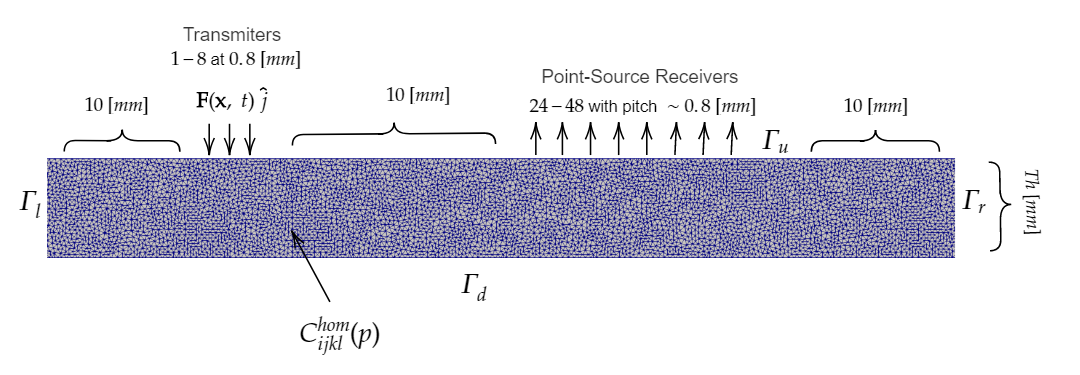
\includegraphics[width=\textwidth]{images/ImgExt/SimP5TransIso12M780-MeshFile.png}
	\caption{Schematic setting of the numerical model to simulate. It contains the \textit{Dirichlet} and \textit{Neumann} boundary conditions for the elastodynamic problem. The mesh is done using \texttt{CGALs} library.}
	\label{MeshFile2D}
\end{figure}

Moreover, figure (\ref{Sim2D-TimeStep}) describes an explicit time-step of simulation, it shows in particular the propagated wave-front with their symmetric and anti-symmetric profiles.
\begin{figure}[!h]
	\centering
	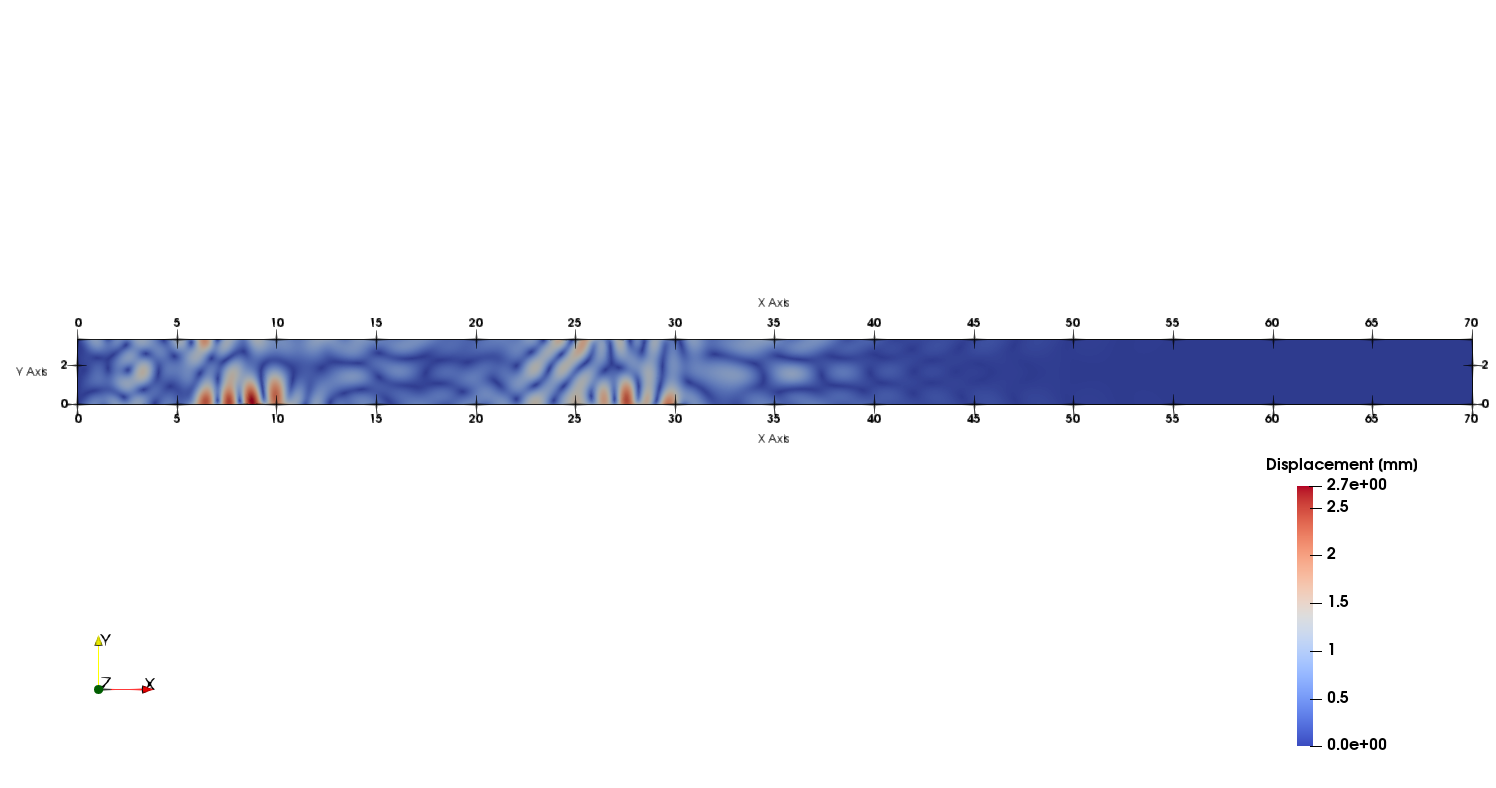
\includegraphics[width=\textwidth]{images/ImgExt/SimP6TransIso33M780T310.png}
	\caption{Simulated wave-guide stopped at time $31 [\mu s]$. It shows in colors the intensity of the propagation wave along the rectangular domain and the interaction with the mixed boundary conditions imposed. This case is parametrized by $(6\%, 3.3 [mm])$ porosity-thickness pair.}
	\label{Sim2D-TimeStep}
\end{figure}



\subsection{Case of Multiple Sources}
Its simulated under the setting of 8 force sources activated independently, i.e., one at each experimental simulation, thus defining 8 different wave-guided propagation of the model (\ref{HomPDE-Simulation}).

\begin{rem}
The computation times associated to the multiple-cases setting vary according to the thickness parameter, since it defines the mesh size. Using a test size of $40 \, [\mu m]$ for the diameter of the cells within the mesh, the simulation times for different cases varies between $\sim 16-28$ hrs in the range of thicknesses $1-3 \, [mm]$. Moreover, it is found experimentally a quadratic time increment depending on the mesh size, for which a testing case at $20 [\mu m]$ takes $\sim 5-7$ days. 
Therefore it was necessary to consider particular properties of the wave propagation to reduce the computational times for each simulation.
\end{rem}

The figure (\ref{FK-DiagramS8P12M10}) describes the \textit{Lamb}-curves obtained from the numerically simulated $(f,k)$-diagram. It shows the validation of the implemented model with respect to the theoretical prediction curves, observing clear correspondence between symmetrical and anti-symmetrical modes.

\begin{figure}[!h]
	\centering
	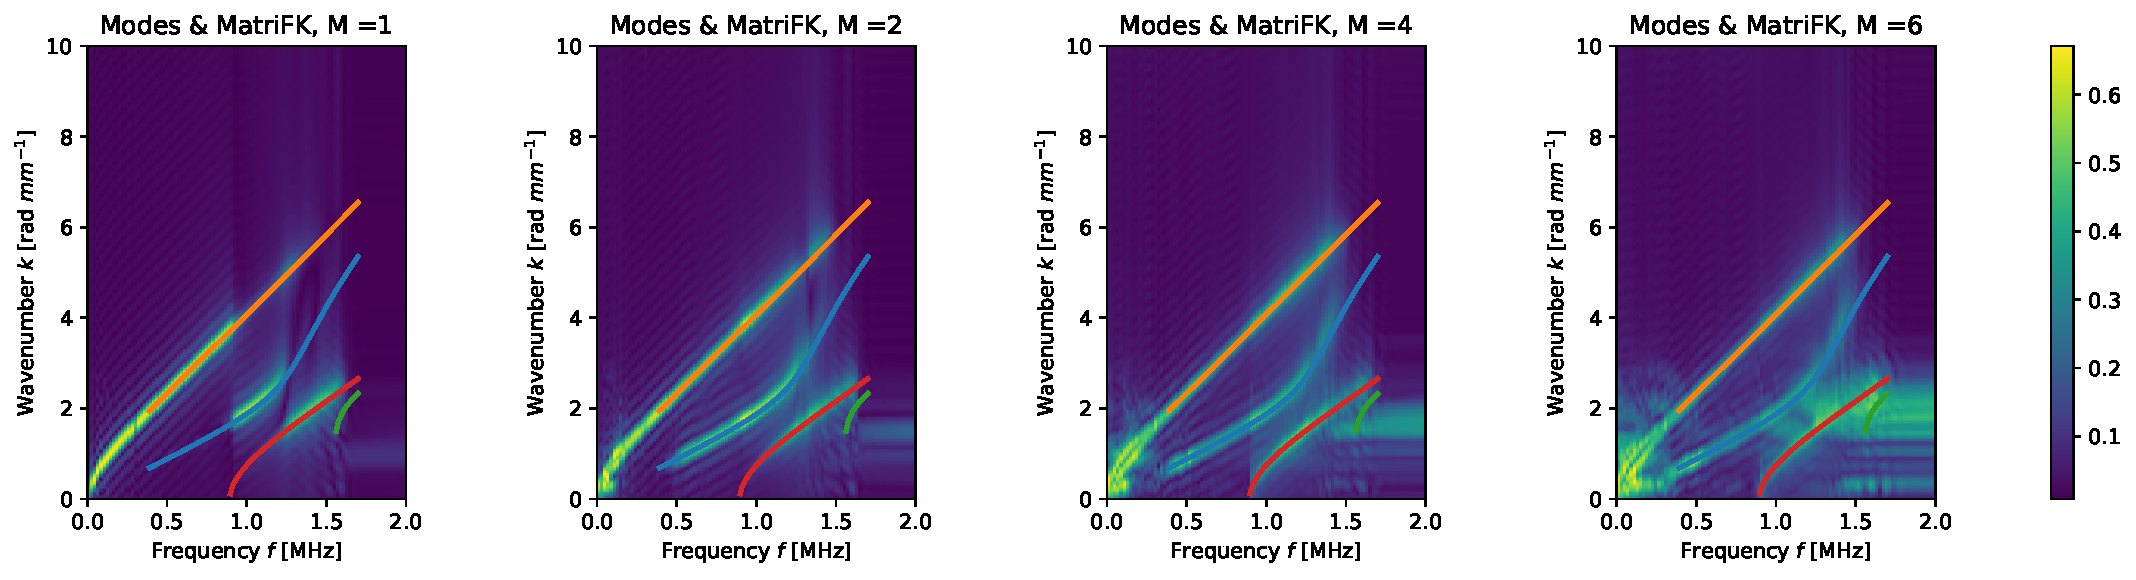
\includegraphics[width=\textwidth]{images/TimeMultSous/2DTimeS8P12ElasticFK10M780_y.pdf}
	\caption{Numerically Simulated $(f,k)$-diagram of a 2D transverse elastodynamic model, Setting of 8 sources with $12\%$ porosity and thickness of $1.0 [mm]$, with the mesh at $40 \, [\mu m]$ of cell inner diameter.}
	\label{FK-DiagramS8P12M10}
\end{figure}

Similarly (\ref{SVD-S8P12M10}) describes the modes in $[dB]$ from the singular value decomposition of the recorded array. It shows the preponderance of the first three modes describing the wave-front.

\begin{figure}[!h]
	\centering
	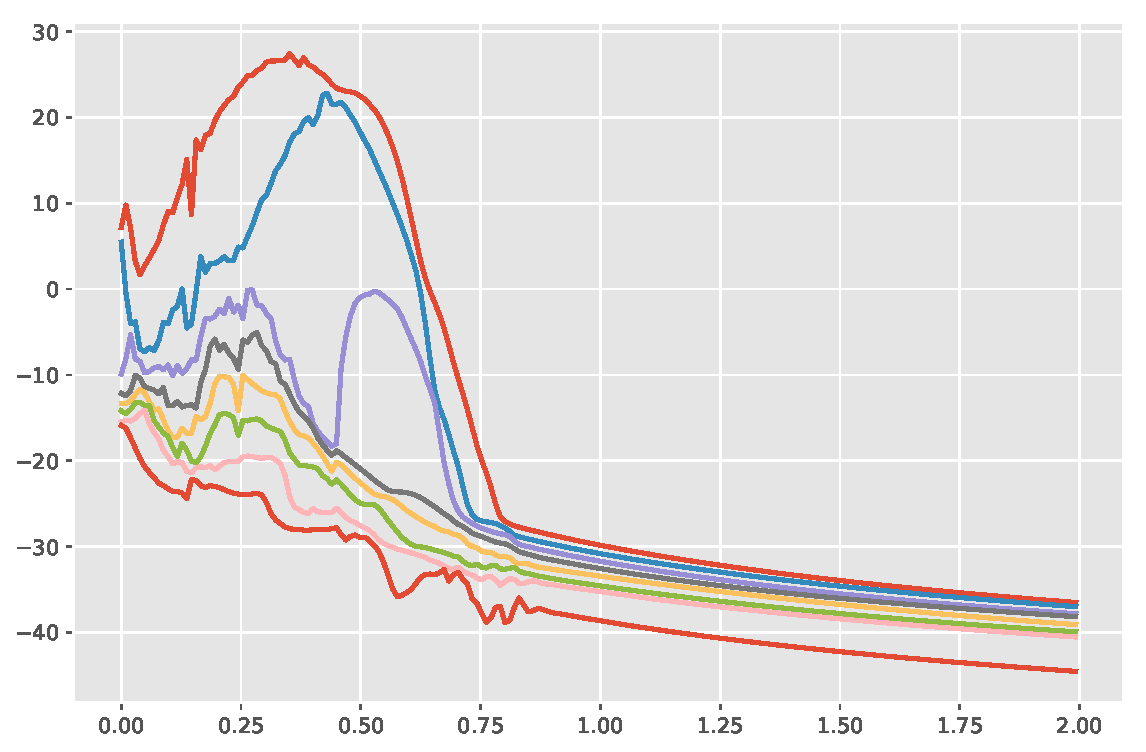
\includegraphics[scale=.5]{images/TimeMultSous/2DTimeS8P12Elastic10_SV.pdf}
	\caption{Singular values obtained by the SVD decomposition of the recorded signal from the simulation \ref{FK-DiagramS8P12M10}}
	\label{SVD-S8P12M10}
\end{figure}

The presence of several symmetric and anti-symmetric modes expressed by the \textit{Lamb} waves is related experimentally with higher thickness values, since in this case the range of horizontal propagation is bigger.
Under such consideration, its shown on figure (\ref{FK-DiagramS8P3M28}) the wave-front simulations for a different pair $(Th., Po.)$, displaying a greater number of prediction curves.

\begin{figure}[!h]
	\centering
	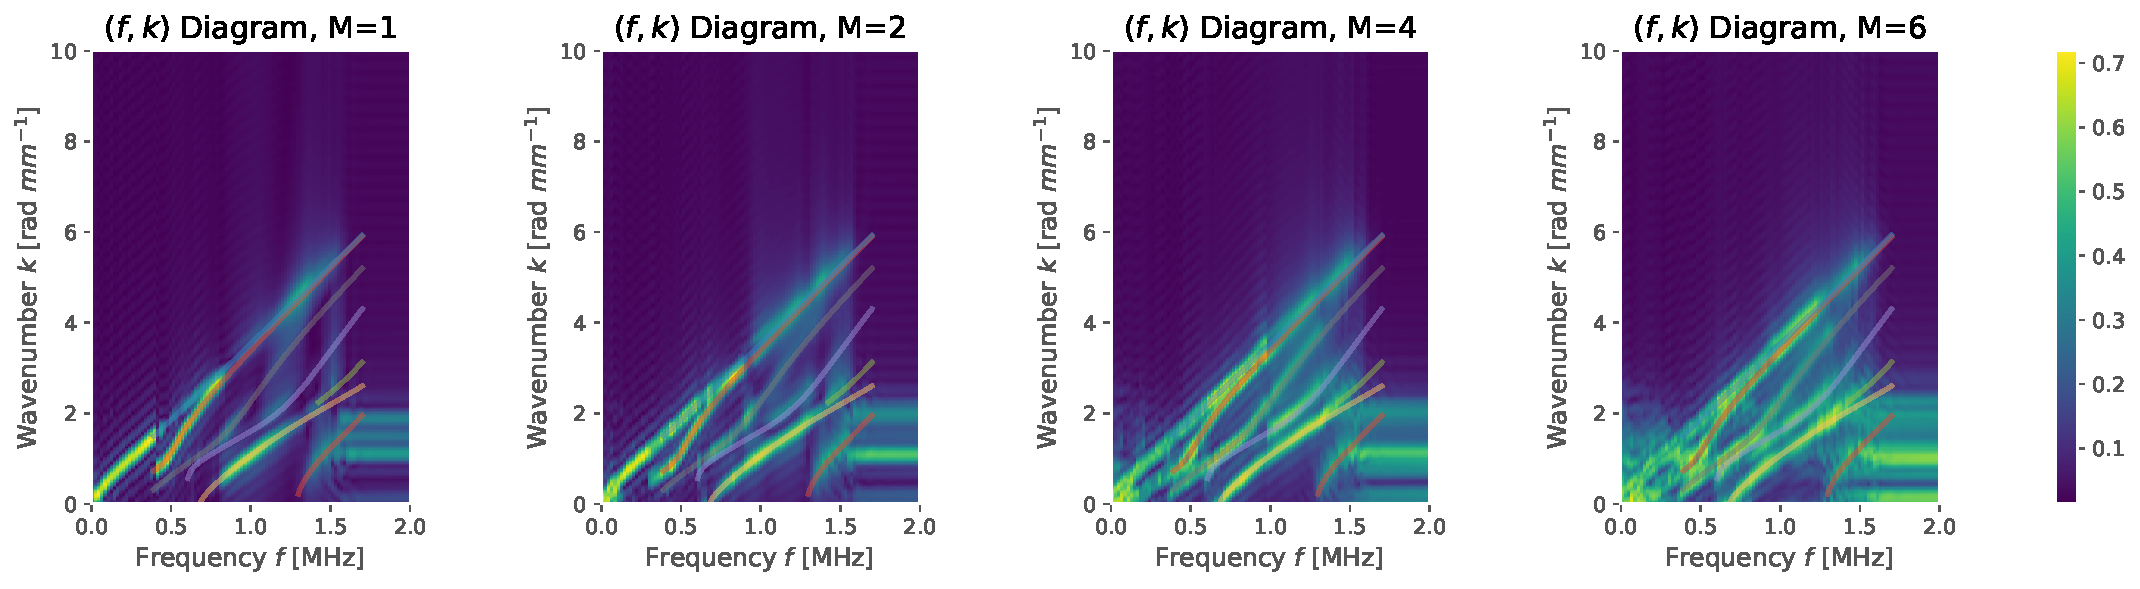
\includegraphics[width=\textwidth]{images/TimeMultSous/2DTimeS8P3ElasticFK28M780_y.pdf}
	\caption{Numerically Simulated $(f,k)$-diagram of 2D transverse elastodynamic model. Setting of 8 sources with $3\%$ porosity and thickness of $2.8 [mm]$.}
	\label{FK-DiagramS8P3M28}
\end{figure}

Similarly, the corresponding modes in $[dB]$ from the singular value decomposition of the recording signal is shown on (\ref{SVD-S8P3M28}), that compares naturally to the experimental reference literature.

\begin{figure}[!h]
	\centering
	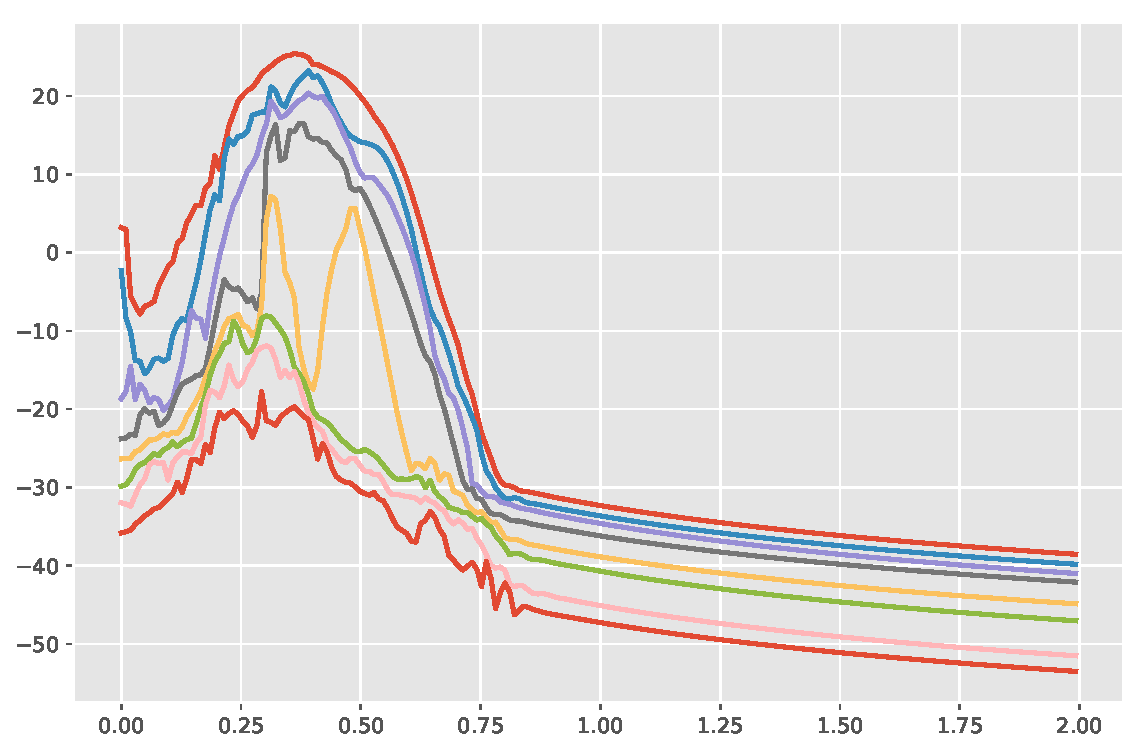
\includegraphics[scale=.5]{images/TimeMultSous/2DTimeS8P3Elastic28_SV.pdf}
	\caption{Singular values obtained by the SVD decomposition of the recorded signal from the simulation \ref{FK-DiagramS8P3M28}}
	\label{SVD-S8P3M28}
\end{figure}



\subsection{Case of a Single Source}
The above study of simulations with a 8-source input force to generate one sample of data introduce problems of computation under limited resources and time. 
To tackle such problem its used the space invariance of the elastic wave, since essentially, the excitation produced by a particular force-source defines a wave-front that propagates throughout the receivers varying only the position of each one of the 8 input forces, thus the recording generated from each force are defined by spatial translation of the wave-front. Therefore by the homogeneity and symmetry of the domain being used, and the parameter independence of the domain, the 8-source setting can be exchanged to a one-source force with a higher number of receivers. This setting produces a lowering of the time require to generate a full simulation, explicitly lowering to 1/8 of the initial time, but introducing reflection effects produced by the boundary conditions that affect the wave-front and modify it.

\begin{rem}
Under this setting of one-source force, it is simulated for the mesh with cell diameters of $\sim 20 \, [\mu m]$ describing high-fidelity results with respect to the inverse problem prediction. The simulation times range with respect to the thickness describing the mesh, in which under a cores of a Xeon E5-2660 v2 processor with 4 Gb. DRR3 RAM requiring $\sim 18-26$ hrs. to describe a full simulation using $1024$ time step associated to $51.2 [\mu s]$ of real-time experimentation.
\end{rem}
It's shown then on figure (\ref{FK-DiagramS1P6M33}) the $(f,k)$-diagram associated to the 1-source simulations of a particular setting. It presents natural reflections related to the rectangular 2-dimensional domain used with mixed boundary conditions.
\begin{figure}[!h]
	\centering
	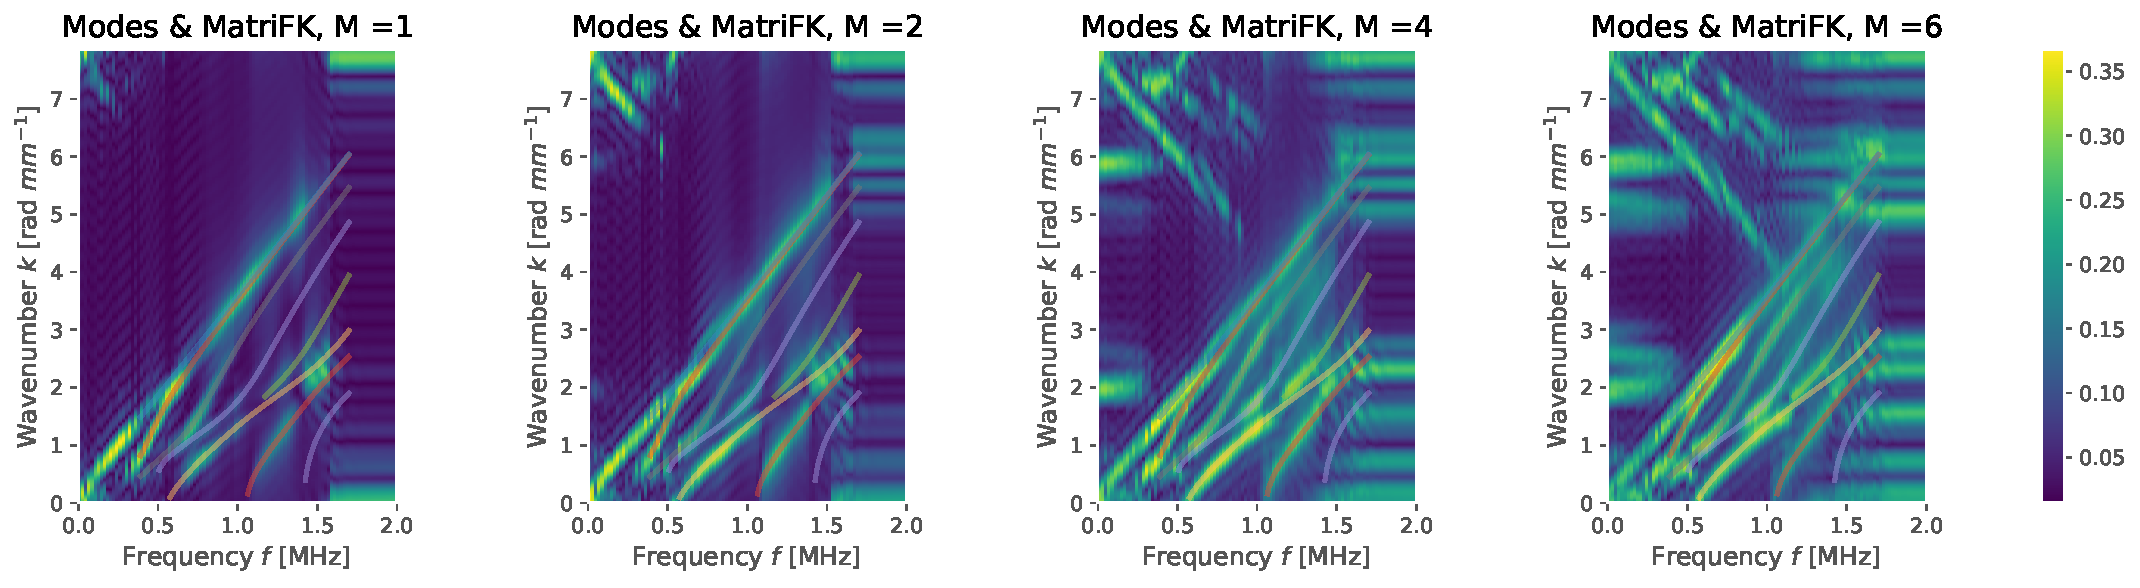
\includegraphics[width=\textwidth]{images/TimeSingSous/2DTime_P6ElasticFK33M1460_y.pdf}
	\caption{Numerically Simulated $(f,k)$-diagram of 2D transverse elastodynamic model. Setting of 1 source with $6\%$ porosity and thickness of $3.3 [mm]$.}
	\label{FK-DiagramS1P6M33}
\end{figure}

Moreover, figure (\ref{SVD-S1P6M33}) describes the main modes associated to the recorded signal, following a realistic order of magnitude and oscillatory sine-like form characteristic from the input signal being used.
\begin{figure}[!h]
	\centering
	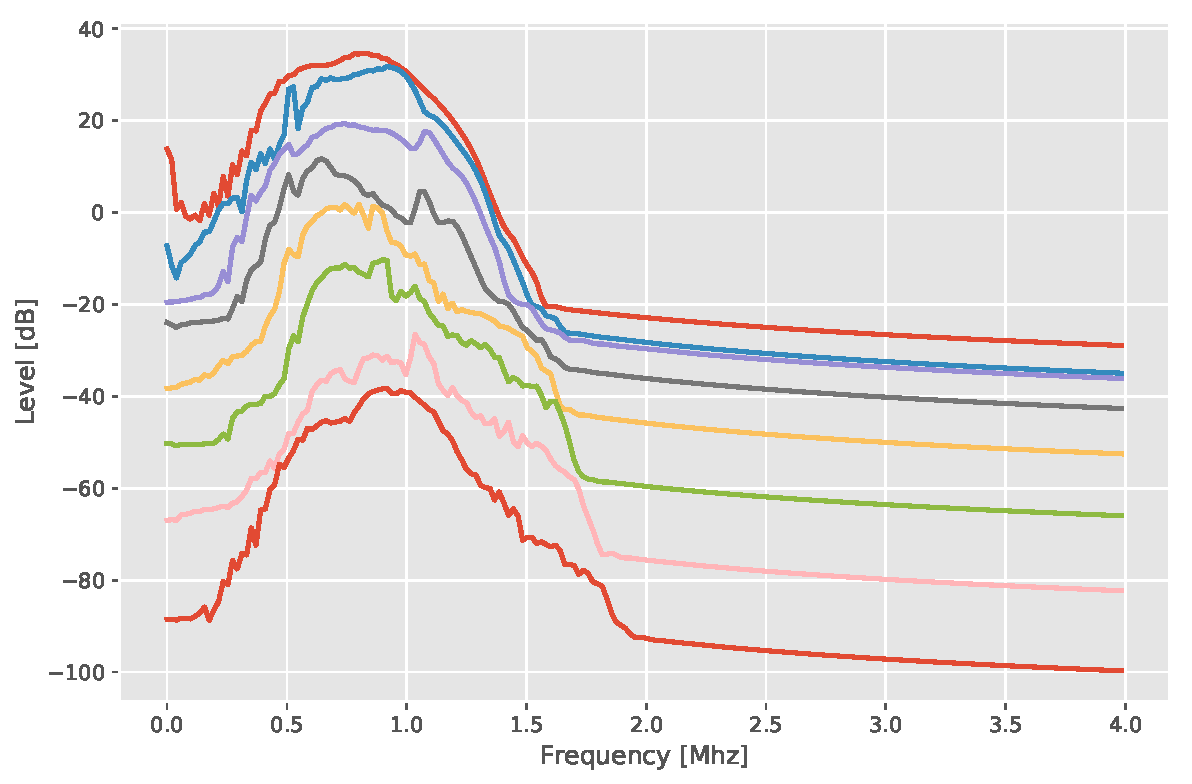
\includegraphics[scale=.5]{images/TimeSingSous/2DTime_P6Elastic33_SV.pdf}
	\caption{Singular values obtained by the SVD decomposition of the recorded signal from the simulation (\ref{FK-DiagramS1P6M33})}
	\label{SVD-S1P6M33}
\end{figure}

The reflections shown in the image (\ref{SVD-S1P6M33}) produced from the simulations corresponds to an aliasing effect in the input signal $S(f_n, e_m, \mathbf{x}_p)_{(m,p) \in [N^E]\times [N^R]}$ after applying FFT over the space $[N^E] \times [N^R]$. Such aliasing express the folding of the $k$-variable \footnote{Associated to the wavenumber} by the conjugation property on \texttt{FFT}, i.e., 
\begin{equation*}
    \overline{\texttt{FFT}(S(f_n, \cdot, e_m))(k)} := \sum_{m=0}^M S(f_n, \mathbf{x}_p, e_m) \overline{e^{-2 \pi i \frac{p k}{M}}} = \texttt{FFT}(S(f_n, \cdot, e_m))(-k)
\end{equation*}
in such a way that the norm associated is the same. Moreover since we consider a finite wavenumber interval denoted $[0, k_{max}]$, such a reflected wavenumber is given by $k_{max}-k$ as observed in the figure.

Given such a symmetry, its considered the application of the analytic projector defined for a given signal $s$ regular enough by:
\begin{equation*}
    \mathcal{P}(s) := (I + \mathbf{i}\mathcal{H})(s)
\end{equation*}
being $\mathcal{H}$ the Hilbert transform. Such a projector defines the analytic signal of $s$ by constructing its real and imaginary parts.

Since the behavior observed in the $(f,k)$-diagram (\ref{FK-DiagramS1P6M33}) shows symmetry with bigger values of $M$, a natural idea is to use the \textit{Hilbert} transform on the input signal, obtaining a analytic signal which maintains the structure of the \textit{Lamb} modes and moreover recreates experimentally obtained results \textit{in-vivo} and \textit{ex-vivo}.
Applying then such a projection filter we obtain the results qualitatively and quantitatively similar with respect to the real experimental data.

\begin{figure}[!h]
	\centering
	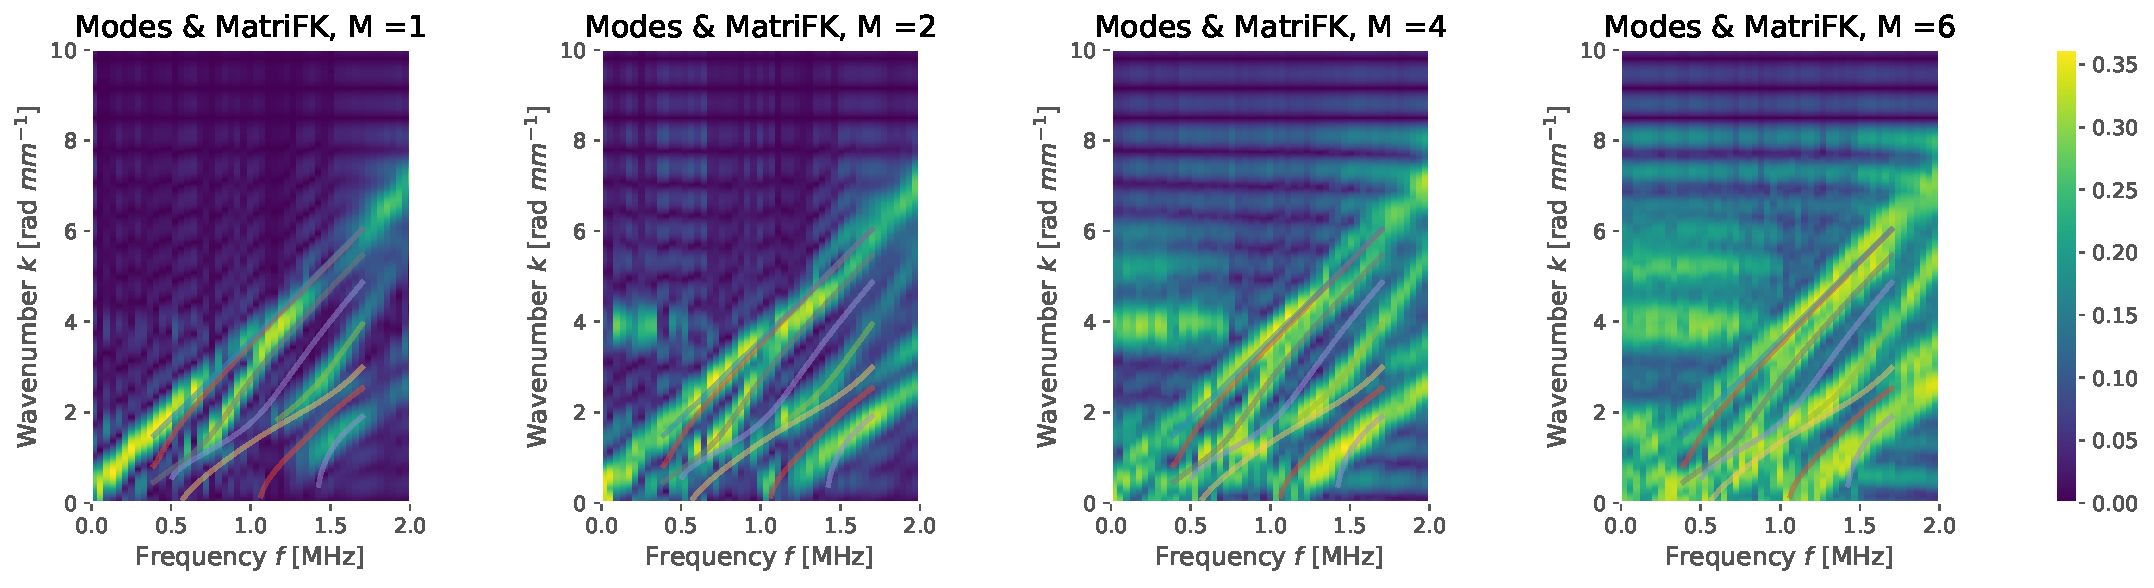
\includegraphics[width=\textwidth]{images/TimeSingSous/2DTimeHilb_P6ElasticFK33M1460_y.pdf}
	\caption{Numerically Simulated $(f,k)$-diagram of 2D Elastodynamic Model: Setting of 1 source with $6\%$ porosity and thickness of $3.3 [mm]$ appplying Hilbert transform to delete reflexions.}
	\label{FK-Hil-DiagramS1P6M33}
\end{figure} 

\begin{figure}[!h]  
	\centering
	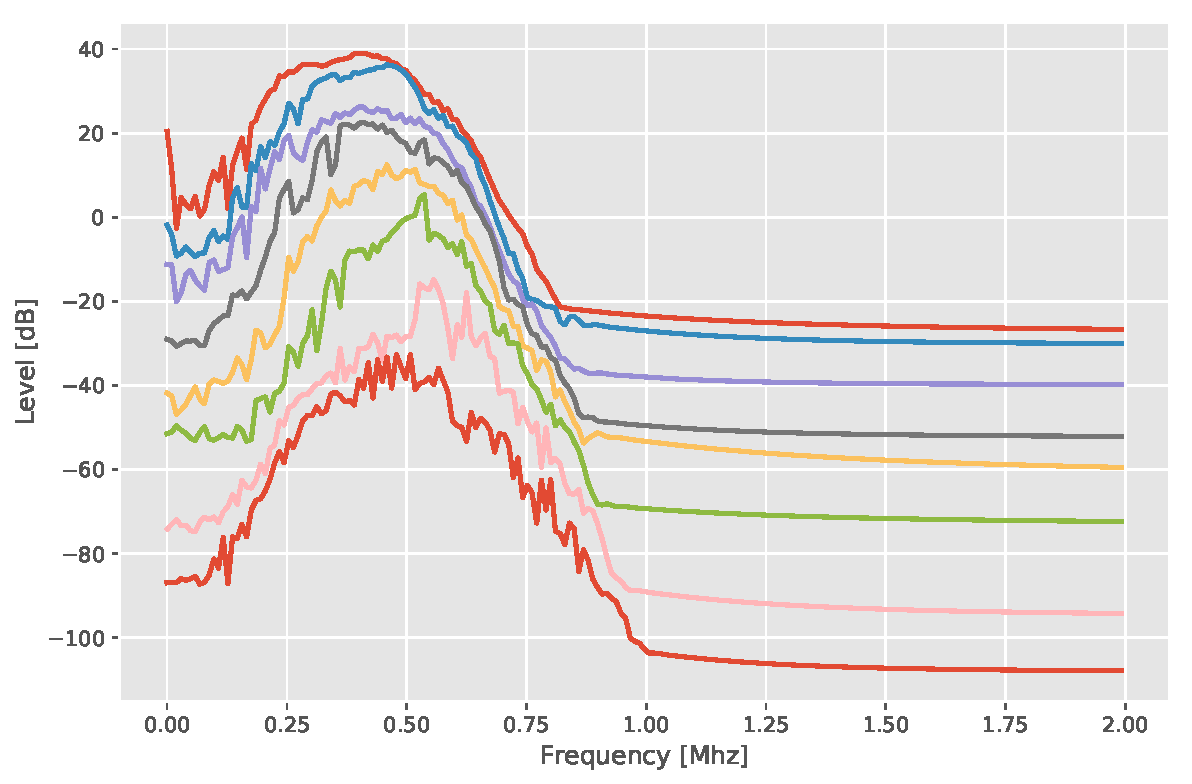
\includegraphics[scale=.5]{images/TimeSingSous/2DTimeHilb_P6Elastic33_SV.pdf}
	\caption{Singular values obtained by the SVD decomposition of the recorded signal from the simulation \ref{FK-Hil-DiagramS1P6M33}}
	\label{SVD-Hil-S1P7M33}
\end{figure}

To give statistical results, using uniformly distributed pairs in the parameters space of biomedical interest it is simulated under the above setting, obtaining the following results in terms of Root Mean Square Error (RMSE), validating the model used and the simulations being done.

\begin{table}[!h]
\centering
    \begin{tabular}{l l l}
    \toprule
    \textbf{RMSE} & \textbf{Porosity} (0-30 \%) & \textbf{Thickness} (1-4) [mm]\\
    \midrule
    Axial Meas. & 0.87 \% & 0,02  [mm]\\
    Anti-Axial Meas. & 0.47 \%  & <0.01 [mm]\\
    Composed & 1.2 \% & 0.03 [mm] \\
    \bottomrule
    \end{tabular}
    \caption{RMSE results from time-domain simulations using a set of 8 (porosity, thickness) pairs homogeneously distributed on the space of biomedical interest. Explicitly, the \textbf{Axial Meas.} defines vertical measurements of displacement, \textbf{Anti-Axial Meas.} defines horizontal measurement of displacement, whereas \textbf{Composed} defines measurement of maximum values between each of the two above, thus being of mixed type.} 
    \label{TimeInvTable}
\end{table}

A critical aspect regarding the experimental procedure is defined by the device sensitivity towards axial measurements. It has been observed that small variations of the device alignment implies corrupted recording that produce therefore wrong (porosity, thickness) prediction pairs.
In this sense, table (\ref{TimeInvTable}) shows explicitly the direction-sensibility dependence towards the recordings. As Axial and Anti-axial measurement itself retrieve RMSE lower enough in biomechanical settings, the compose recordings of data, retrieve porosity errors order of magnitude higher. Thus, directional data contamination compromise robustness of the inverse problem formulation. Therefore, an aspect that must be considered from the modelling setting as in the experimental device.


\section{Case on Frequency Domain}

The time-domain simulation given results which represent qualitatively the model with enough fidelity, nevertheless such simulation requires a relatively small time step in such a way that the full simulation take considerable time. Thus, it is necessary to consider a model which reduces the computational cost.
To this end, taking into account that the signal processing involves the application of \texttt{FFT} over the sensors data, a straightforward method is to consider the simulations now in the time-domain over the arrays of frequencies that are of interest.

\subsection{Solutions without Attenuation}
In this case, using the schemes proposed in the section before, its show results in which \textit{Lamb}-waves contained unnatural discontinuities passing from a symmetric mode to an anti-symmetric one, also $dB$ values ranging with over $10$ orders of magnitude. Such distortion are shown in (\ref{FK-Freq-DiagramS8P10M09}) and (\ref{SVD-Freq-S8P10M09}) respectively. This kind of behavior repeated over different pairs of porosity level under study ranging the full domain of biomedical interest associated to the simulations thus becoming an intrinsic aspect of the elastic operator under study.

\begin{figure}[!h]
	\centering
	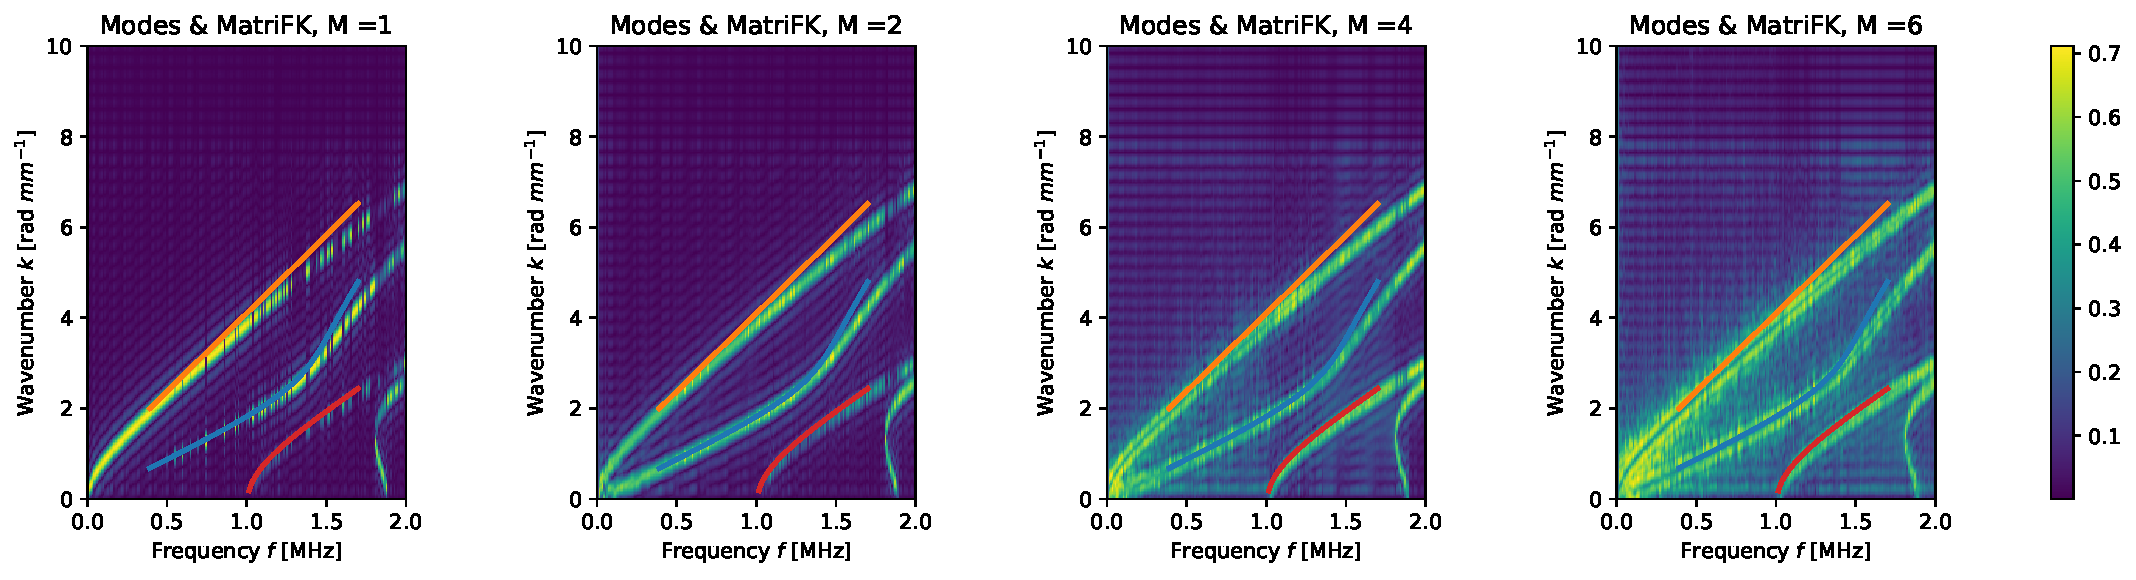
\includegraphics[width=\textwidth]{images/FreqRes/2DFreqS8P10ElasticFK09M300_y.pdf}
	\caption{Numerically simulated $(f,k)$-diagram of 2D Elastic Model on Frequency Domain: Setting of 8 sources with $10\%$ porosity and thickness of $0.9 \,[mm]$}
	\label{FK-Freq-DiagramS8P10M09}
\end{figure} 

\begin{figure}[!h]
	\centering
	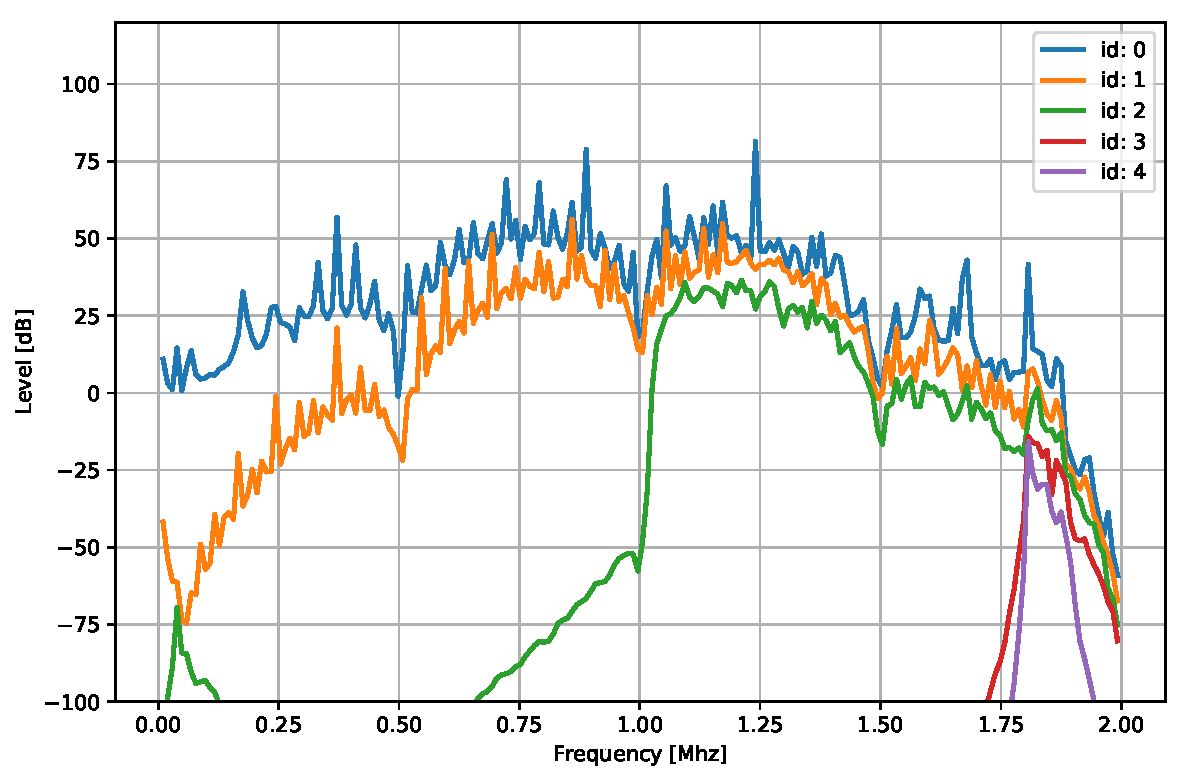
\includegraphics[scale=.5]{images/FreqRes/2DFreqS810Elastic09_SV.pdf}
	\caption{Singular values obtained by the SVD decomposition of the recorded signal from the simulation \ref{FK-Freq-DiagramS8P10M09}.}
	\label{SVD-Freq-S8P10M09}
\end{figure}


Nevertheless, several sets of simulations are done to study and validate the wave-front generated. The table (\ref{FreqInvTable}) shows the RMSE results where the predictions are done using an optimization algorithm to fit the recorded data to a set of references, i.e., solving the inverse problem \cite{Minonzio2018}. The results shows validation of the frequency domain simulations even with the discontinuities observed both in the $(f,k)$-diagram as in the multiple peaks observed on (\ref{SVD-Freq-S8P10M09}). Such results can be explained from the clear behavior shown even at high-frequencies, thus enabling a clear fitting of the \textit{Lamb}-curves even with discontinuities of the processed signal.
\begin{table}[!h]
\centering
    \begin{tabular}{l l l}
    \toprule
    \textbf{RMSE} & \textbf{Porosity} (0-30 \%) & \textbf{Thickness} (1-4) [mm]\\
    \midrule
    Axial Meas. & 1.15 \% & 0,03  [mm]\\
    Anti-Axial Meas. & 1,11 \%  & < 0,01 [mm]\\
    Composed & 0.8 \% & 0.02 [mm] \\
    \bottomrule
    \end{tabular}
    \caption{RMSE results from frequency-domain simulations using a set of 8 (porosity, thickness) pairs homogeneously distributed on the space of biomedical interest. Explicitly, the \textbf{Axial Meas.} defines vertical measurements of displacement, \textbf{Anti-Axial Meas.} defines horizontal measurement of displacement, whereas \textbf{Composed} defines measurement of maximum values between each of the two above, thus being of mixed type.}
    \label{FreqInvTable}
\end{table}

The presence of discontinuities observed on the curves from  the $(f,k)$-diagram (\ref{FK-Freq-DiagramS8P10M09}) as in the peaks shown on (\ref{SVD-Freq-S8P10M09}) describes a non-natural behavior of the wave-front. Multiple possible causes can be attributed to such effect, ranging from resonance behavior of the mesh itself, discontinuity effects of the discretization procedure or the bad-possedness of the elastic operator itself.

In this particular case, let us recall from the justification section, that the existence results of the elastodynamic solution is derived from the existence of an increasing sequence of eigenvalues associated to the elastic operator (\ref{EigenValuesProp}). In this context, such eigenvalues will be called eigen-frequencies and they correspond to the main cause of such discontinuities observed before on the simulations as will be studied in what follows.

Such a study corresponds to the formulation of an eigenvalue problem associated to the elastic operator, defined as finding the pairs $\{(\lambda_k, u_k) \, : \, k \in \mathbb{N} \} \subset \mathbb{R}_+ \times \mathbf{H}^1(\Omega, \Gamma_D)$ solution to the following variational form:

\begin{equation*}
    \label{VariationalEigenProb}
    \mathcal{I}_{\mathbf{C}^{hom}} (u_k, v) = \lambda_k (u_k, v)_{\Omega} \quad \forall v \in \mathbf{H}^1(\Omega, \Gamma_D)
\end{equation*}
where we identify each eigenvalue to the eigenfrequency associated to our problem in the form:
\begin{equation*}
    \lambda_k = \rho^0 (2\pi f_k)^2, \text{ i.e. } f_k = \frac{1}{2\pi} \sqrt{\frac{\lambda_k}{\rho^0}} \quad k \in \mathbb{N}_{*}
\end{equation*}

\begin{rem}
Let us note in particular that the existence of such pairs is obtained from a classical result of elliptic theory \cite{raviart1983introduction}, \cite{evans2010partial}. Explicitly, it follows since the homogenized coefficients are elliptic and moreover they are bounded which gives us a well-defined bilinear, bicontinuous and coercive operator $\mathcal{I}_{\mathbf{C}^{hom}}(\cdot, \cdot)$ and a linear continuous operator $b(\cdot) := (u_k, \cdot)$ defined respectively on $\mathbf{H}^1(\Omega, \Gamma_D)\times \mathbf{H}^1(\Omega, \Gamma_D)$ and $\mathbf{H}^1(\Omega, \Gamma_D)$.
\end{rem}


By solving the problem (\ref{VariationalEigenProb}), it was found a discrete spectrum with abundant eigen-frequencies in bounded intervals of frequency as predicted from (\ref{EigenValuesProp}), nevertheless the experimental frequency array which was necessary to use for further studies in connection with the real data showed a neighborhood of at least eigen eigen-frequencies over each experimentally selected frequency. 

In (\ref{EigenValuesComparison}) is shown the frequencies used in the experimental setting used for the simulations in the frequency domain and the eigen-frequencies associated to the operator under study. It explicitly describes the correspondence of the found eigen-values within a close neighborhood of the simulated frequency array and moreover, intersecting the peaks with resonance modes, thus explaining the resonance and un-natural discontinuity effect observed before.

\begin{figure}[!h]%
    \centering
    \subfloat[Start Bandwidth]{{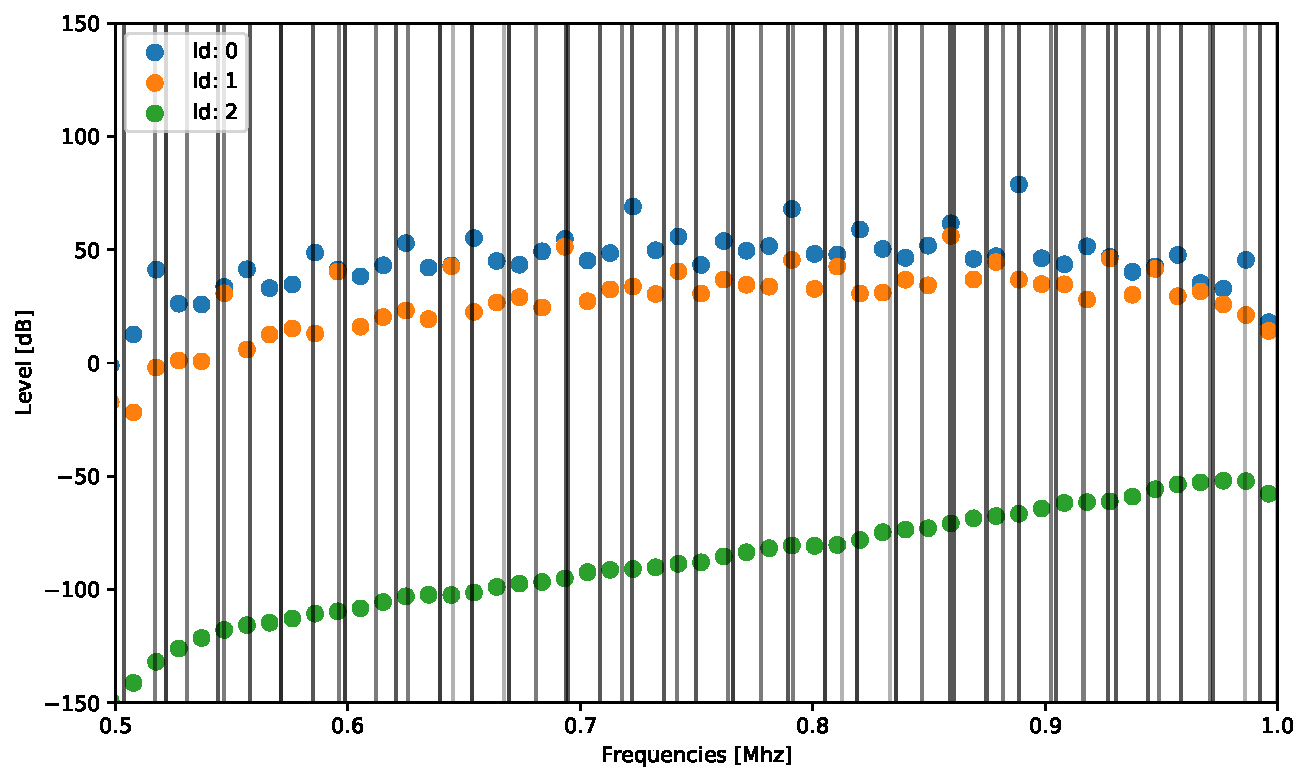
\includegraphics[width=7cm]{images/FreqRes/SingValues-EigenFreqs05-10.pdf} }}%
    \qquad
    \subfloat[End Bandwith]{{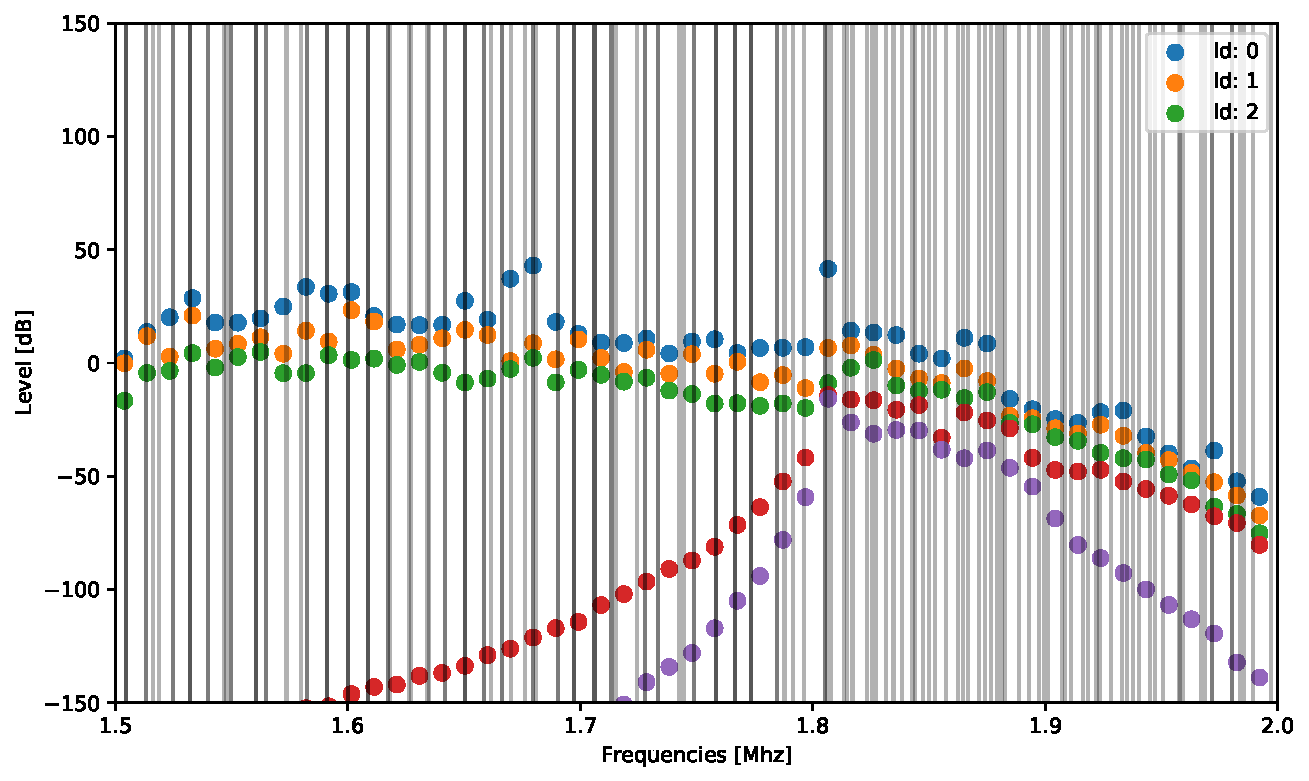
\includegraphics[width=7cm]{images/FreqRes/SingValues-EigenFreqs15-20.pdf} }}%
    \caption{Comparison between Singular Values and Eigen-frequencies: Experimentally its found a increasing sequence of eigenvalues that intersects the experimentally chosen array frequencies.}%
    \label{EigenValuesComparison}%
\end{figure}


\subsection{Solution using Attenuation.}
To bypass the oscillation observed at the frequency-domain problem, its considered adding a $\epsilon$ viscous-like term, such model in particular defines a translation of the eigen-frequencies from the elastic operator to the complex plane, thus avoiding the real plane resonances. In this sense, is expected an smoothing effect on the real part recordings, and moreover this implies avoiding the ill-conditioned matrix system from the FEM space discretization procedure.

For a fix frequency $\omega \in \mathbb{R}$, let us consider solutions in the form: $u(\mathbf{x},t) = e^{2 \pi i \omega t}\hat{u}(\mathbf{x})$, so that $\hat{u}(\mathbf{x})$ solves the equivalent problem in the frequency domain
\begin{equation*}
    \left \{
    \begin{array}{cc}
        -(2\pi \omega)^2 \rho^{hom} \hat{u}(\mathbf{x}) - i \epsilon \hat{u}(\mathbf{x}) - \nabla \cdot \sigma(\hat{u}) = \mathbf{0} & \text{ in } \Omega \times (0,T) \\
        \sigma^{hom}(\hat{u}(\mathbf{x}))  =  C_{ijkl}^{hom}\mathbf{e}_{kl}(\hat{u}) & \text{ in } \Omega \times (0,T)\\
        \hat{u} = \mathbf{0} & \text{ on } \Gamma_D\times (0,T)\\
        \sigma^{hom}(\hat{u}) \cdot n = \mathbf{F}(\mathbf{x}, \omega) & \text{ on }\Gamma_N \times (0,T)
    \end{array}
    \right .
\end{equation*}
Taking into account that \texttt{FEniCS} version 2017.2.0 doesn't support the usage of a complex coefficient formulation in the variational form, its decomposed the solution in their real and complex part as $\hat{u} = \hat{u}_R + i \hat{u}_I$. It follow then a coupled system satisfied for the pair $(\hat{u}_R, \hat{u}_I)$ given in the form:
\begin{equation*}
    \left \{
    \begin{array}{cc}
        -(2\pi \omega)^2 \rho^0 \hat{u}_R +  \omega \epsilon \hat{u}_I - \nabla \cdot \sigma (\hat{u}_R) = \mathbf{0} & \text{ in }\Omega \times [0,T] \\
        -(2\pi \omega)^2 \rho^0 \hat{u}_I - \omega \epsilon \hat{u}_R - \nabla \cdot \sigma (\hat{u}_I) = \mathbf{0} & \text{ in }\Omega \times [0, T] \\
        \hat{u}_R, \hat{u}_I = \mathbf{0} & \text{ on } \Gamma_D \\
        \sigma(\hat{u}_R)\cdot n, \sigma(\hat{u}_I)\cdot n = \hat{\mathbf{F}}_R, \hat{\mathbf{F}}_I & \text{ on }\Gamma_N
    \end{array}
    \right.
\end{equation*}
which can be solved with the standard tools of \texttt{FEniCS} by the usage of a mixed element for the couple system.

Simulating such system shows on figure (\ref{FK-DiagramFreqS8P12M28}) the $(f,k)$-diagram associated to the 8-sources setting. It presents natural reflections related to the rectangular 2-dimensional domain used with mixed boundary conditions.
\begin{figure}[!h]
	\centering
	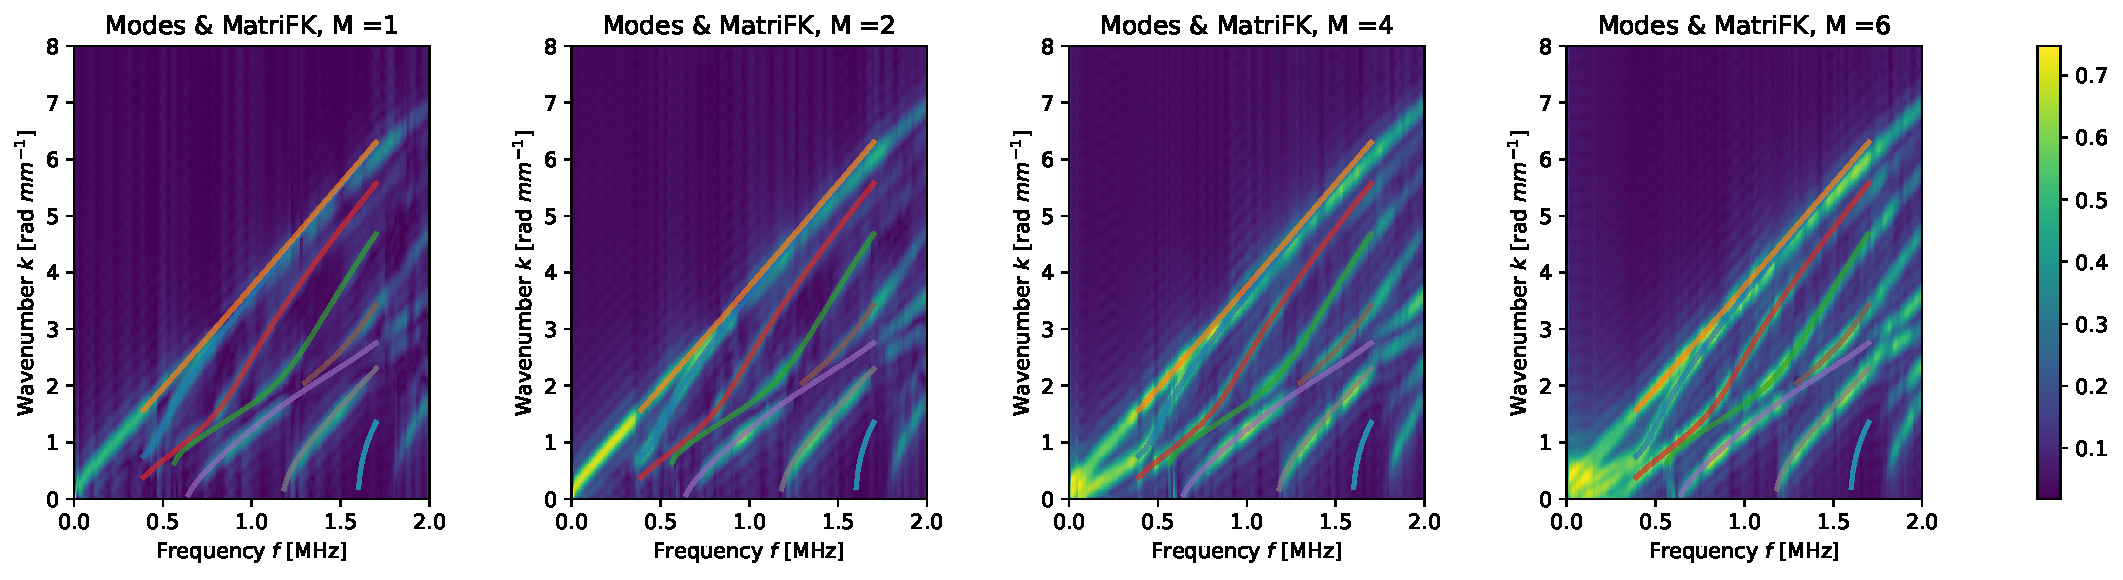
\includegraphics[width=\textwidth]{images/FreqMultSous/2DMixedP12TransIsoFKW28M400_y.pdf}
	\caption{Numerically Simulated $(f,k)$-diagram of 2D Transverse Elastodynamic Model: Setting of 1 source with $3\%$ porosity and thickness of $3.0 [mm]$.}
	\label{FK-DiagramFreqS8P12M28}
\end{figure}

Nevertheless, using figure (\ref{SVD-FreqS8P12M28}) of main modes associated to the recorded signal, its observed vanishing oscillation of the modes, thus numerically avoiding the eigen-frequencies, the main provider of resonances.
\begin{figure}[!h]
	\centering
	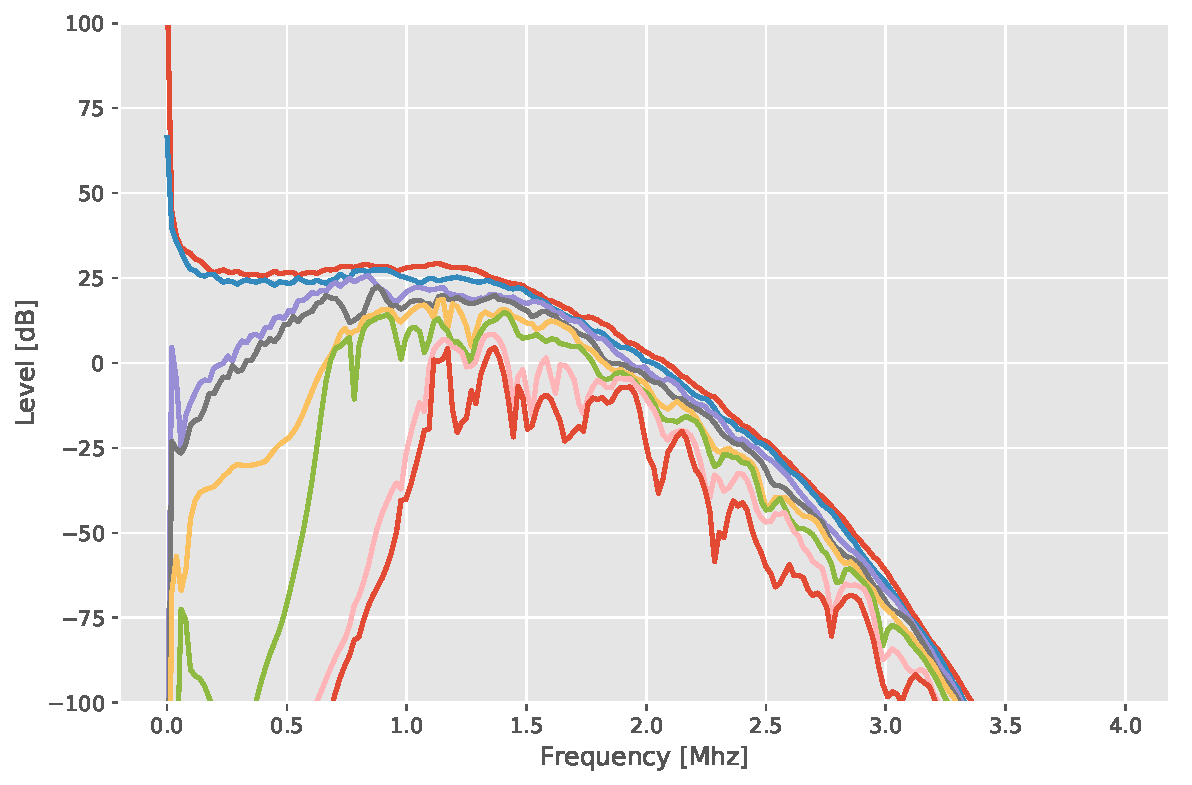
\includegraphics[scale=.5]{images/FreqMultSous/2D-FreqSimP12W28eKV_SV.pdf}
	\caption{Singular values obtained by the SVD decomposition of the recorded signal from the simulation (\ref{FK-DiagramFreqS8P12M28})}
	\label{SVD-FreqS8P12M28}
\end{figure}


\section{3-Dimensional Simulation of Wave Propagation}
Following the 2-dimensional case, it is now studied the effect of radial wave behavior on the recorded signal, assessing in particular the experimentally obtained results that neglect the non-axial wave-guide propagation. In this sense, is assessed the wave-propagation by using a cylindrical type domain characterizing the cortex curvature and on a non-uniform domain derived from $\mu$-CT images that relates the irregularities of inner surfaces from realistic cortical bone samples.
Such procedures imply the creation of adaptive meshes of the complex cortical bone geometry, where open-source software such as \texttt{iso2mesh}, \texttt{CGAL} is used for its generation and in particular is created a pipeline of mesh generation from $\mu$-CT images.

\subsection{Half-Cylinder Case}
A half-cylinder mesh is proposed as first approximation to the 3-dimensional real cortical bone sample from the $\mu$-CT images. In this case, avoiding the non-uniformity characteristic of the bone surface it's tested the wave-guide propagation and distortion generated by the natural curvature of the mesh.

The numerical model setting is schematically proposed on (\ref{HalfCylSubdomainsFile}), resembling the 2-dimensional case (\ref{MeshFile2D}) with variations associated to the input force width and rectangular-type force sensors. Such sensors are modelled to capture now surface forces of type $\sigma^{hom}(u)\cdot n$ restricted to each sensor subdomain. As before, the problem is modelled with \textit{Dirichlet} boundary conditions on $\Gamma_l \cup \Gamma_r$ and \textit{Neumann} condition on $\Gamma_u \cup \Gamma_d$.

\begin{figure}[!h]
	\centering
	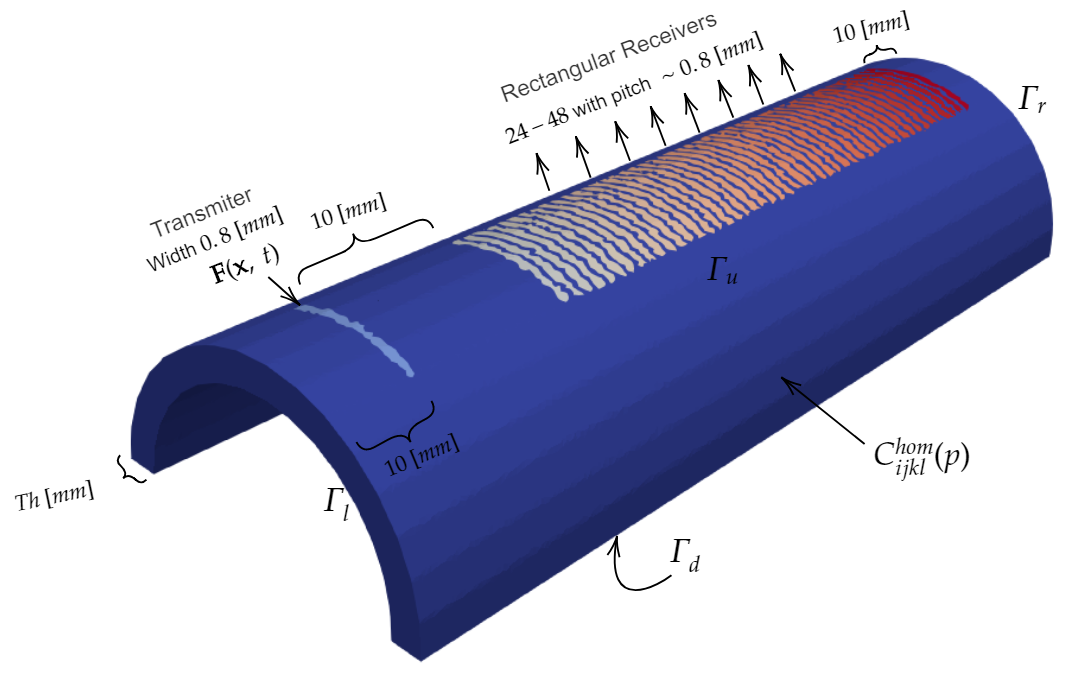
\includegraphics[width=0.8\textwidth]{images/ImgExt/HalfCyl3d-MeshBoundaries.png}
	\caption{Half-Cylinder Mesh defining the geometry for the elastodynamic 1-source simulation with mean diameter of tetrahedral $\sim 40 [\mu m]$. Number of vertices: $176,144$ and number of cells: $956,704$. The colors variations shows the different tagged subdomains describing the numerical implementation and recording on the receptors. In this case, from left to right it's shown source subdomain and force-sensors subdomains in array-like form. }
	\label{HalfCylSubdomainsFile}
\end{figure} 

As before, the implementation is done with \texttt{FEniCS} library on time-domain. Applying a post-processing analysis at particular time step with visual behavior effect is shown on figure (\ref{HalfCyl-TimeStep}) using the \texttt{ParaView} library. The figure describes a wave-front propagating along the axial-plane as expected but with characteristic non-axial behavior not present in 2-dimensional simulations.

\begin{figure}[!h]
	\centering
	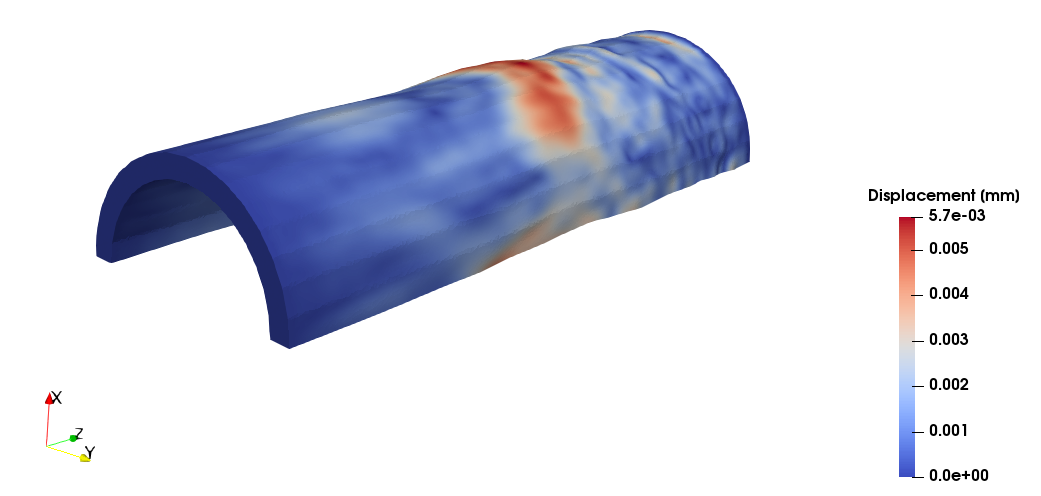
\includegraphics[width=0.8\textwidth]{images/ImgExt/HalfCyl3d-T160.png}
	\caption{Wrapping by vector effect on the simulated domain with input force $\mathbf{F}(\mathbf{x},t)$ at $8 [\mu s]$. The color intensity described by the right-hand side bar shows the magnitude of displacement scaled at $[mm]$. }
	\label{HalfCyl-TimeStep}
\end{figure} 

\begin{rem}
The total simulation time associated to the half-cylindrical mesh is $\sim 25$ hrs. using 2 cores on a Xeon E5-2660 v2 processor with 5 Gb. RAM DDR3. This mesh with cells at $\sim 40 [\mu m]$ defines \textit{Lamb}-waves requiring 1024 time steps partitioning $51.2 [\mu s]$ of real-time simulation. 
\end{rem}

The signal recording from the wave-front propagation partially observed from (\ref{HalfCyl-TimeStep}) enables us to observe the first example of numerically generated \textit{Lamb}-modes characteristic of the \textit{Lamb}-wave theory as shown in (\ref{FK-Cyl-DiagramS1P11M18}). In particular, the 3-dimensional curvature effect from the cortical bone doesn't affect the main three modes, nevertheless anti-symmetrical modes are less clear showing variations respect to the theoretical 2-dimensional theoretical model and vanishing at higher frequencies. On the other hand, symmetrical modes preserve their structure on the central range of frequencies $(0.5, 1.5) [Mhz]$. Moreover, its shown already at level $M=4$ strong reflection effects affecting the signal.
\begin{figure}[!h]
	\centering
	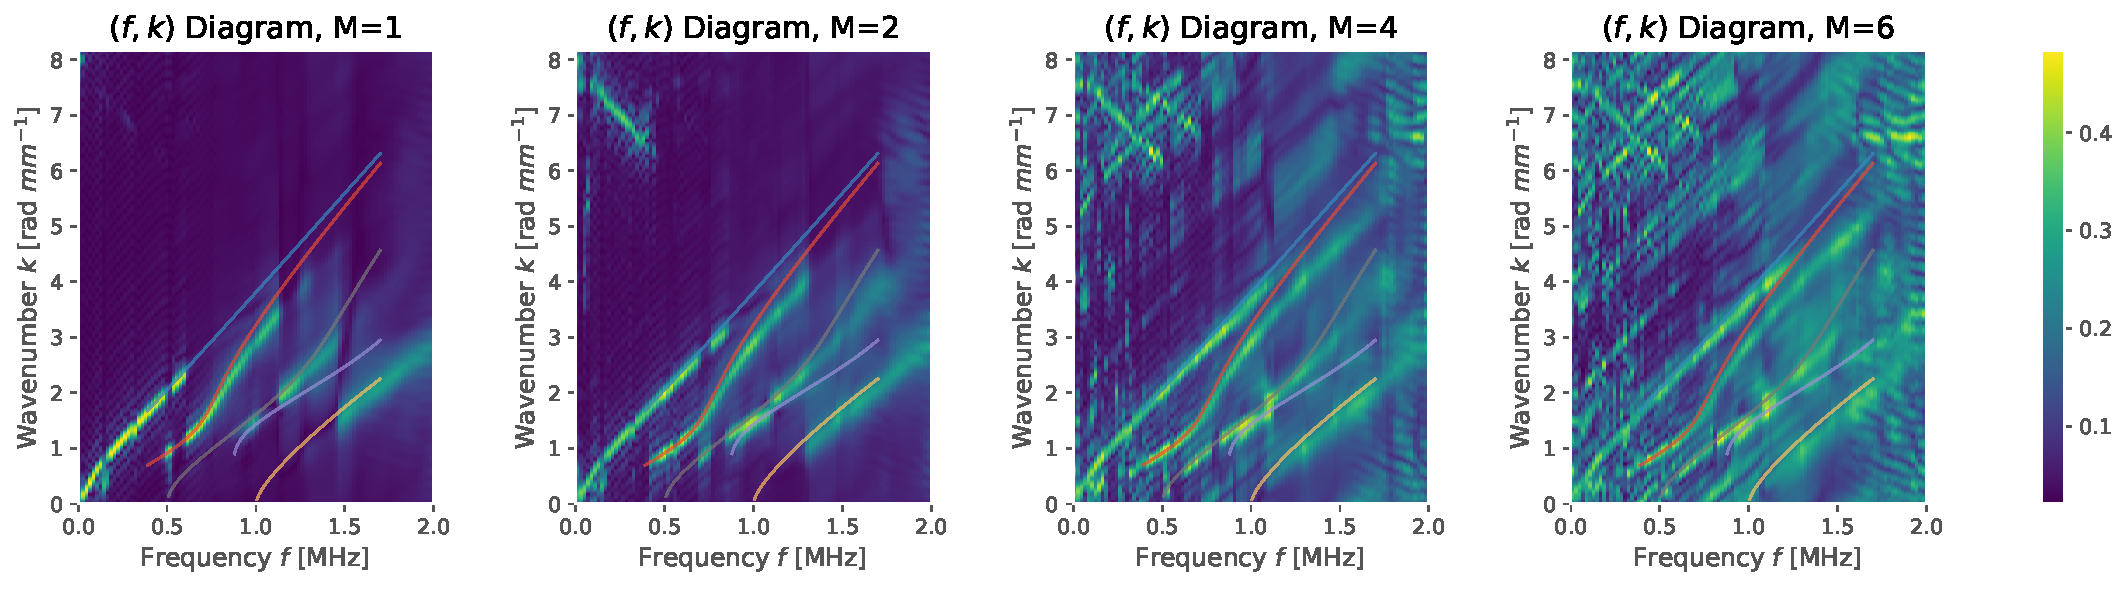
\includegraphics[width=\textwidth]{images/ClusterSim/3DCylTimeP11TransIsoFKW18.pdf}
	\caption{Numerically Simulated $(f,k)$-diagram of a 3-dimensional Half-cylinder Elastodynamic Model: Setting of 1 source with $11\%$ porosity and $1.8 [mm]$ thickness applying Hilbert transform to delete reflections. The inverse formulation retrieves $\sim 1.01\%$ of porosity and $\sim 1.801$ thickness.}
	\label{FK-Cyl-DiagramS1P11M18}
\end{figure} 
With respect to the singular value decomposition of the recorded signal, in figure (\ref{SVD-Cyl-S1P11M18}) the first 3 modes describes a natural behavior in the $(0, 20) \, [dB]$ range associated to the input force currently used. The oscillatory effect is attributed to the sine component on the force-source, decaying at outside the maximum signal intensity at $\sim 5 \, [\mu s]$.
\begin{figure}[!h]  
	\centering
	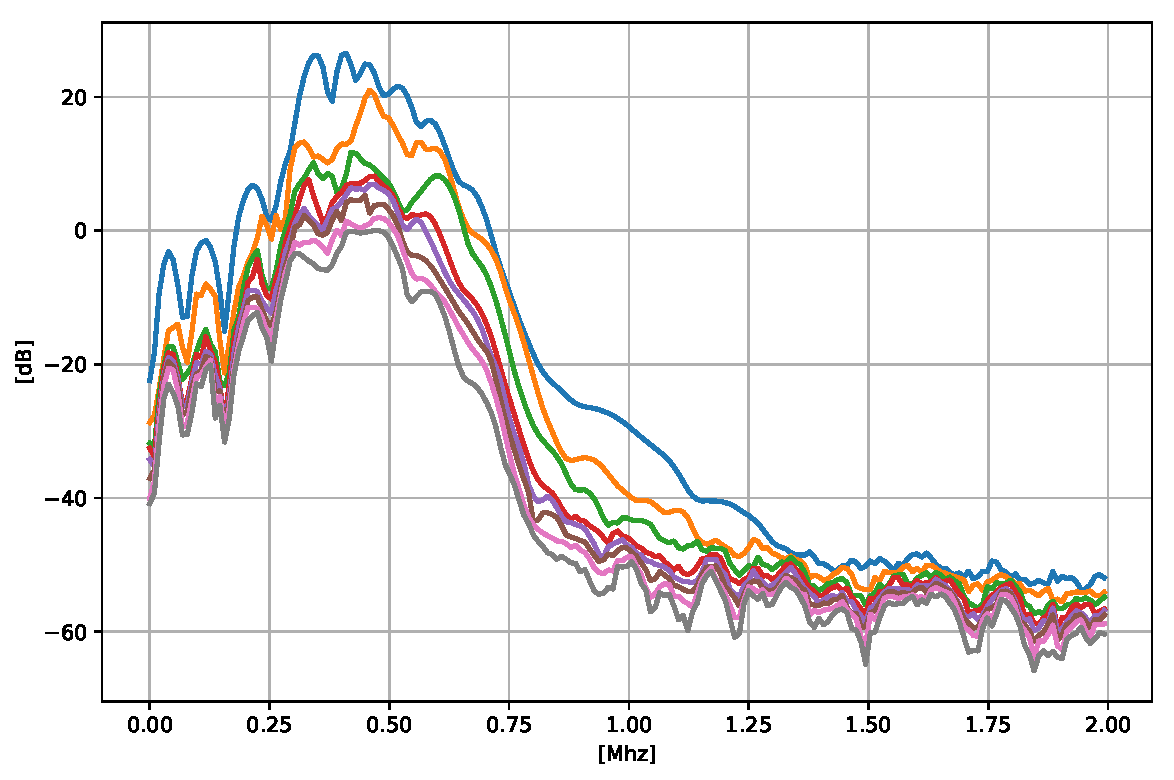
\includegraphics[scale=.5]{images/ClusterSim/3DCylTimeP11TransIsoFKW18_SV.pdf}
	\caption{Singular values obtained by the SVD decomposition of the recorded signal from the simulation (\ref{FK-Cyl-DiagramS1P11M18}). The different modes obtained from the decomposition are shown in different colors, being the first 3 related to the naturally obtain from real \textit{ex-vivo} results.}
	\label{SVD-Cyl-S1P11M18}
\end{figure}


\subsection{Rugous Exterior}
The half-cylinder shows clear correspondence to the 2-dimensional case, showing a prevalence of the axial-propagation over the non-axial effect that occur during the wave-front. Nevertheless, it does not incorporates possible irregularities arising from the constant development of bone being not only the curvature effect relevant to a realistic simulation but also the presence of non-uniform irregularities presented mainly on the infero-interior surfaces on cortical bone samples. In this case, its assessed the mesh creation based on real $\mu$-CT cortical bone images and the data-flow necessary to create a well-defined mesh, simulation and processing of the recordings.

\subsubsection{Mesh Generation}

The mesh generation is done using the data-flow diagram presented in (\ref{DiagramMeshGeneration}). Such procedure works by applying several layer of software's. It creates a complex tetrahedral mesh from a processed volumetric image using as back-end the \texttt{CGAL} library to compute the geometry. 
The processing of the $\mu$-CT gray-scale images stack is defined in three main steps:
\begin{enumerate}
    \item A scaling procedure from the input $9 \, [\mu m]$ voxel images is done to restrict the memory consumption of the full stack of $\mu$-CT images. The output images are obtained with a $56 \, [\mu m]$ voxel, i.e., considering a $40 \%$ scaling factor with cubic interpolator.
    \item The stack is separated between gray-scale value ranges, to isolate the different sets of material involved. In this case, the separation of the mesoscale is done, being the porosities and bone matrix voxel labeled.
    \item Each image labeled set of voxel, is then stacked, defining a volumetric image on \texttt{Octave}, meshed with \texttt{Iso2mesh} library which is a wrapped application containing the \texttt{CGAL} algorithms of mesh generation.
\end{enumerate}
\begin{figure}[!h]
	\centering
	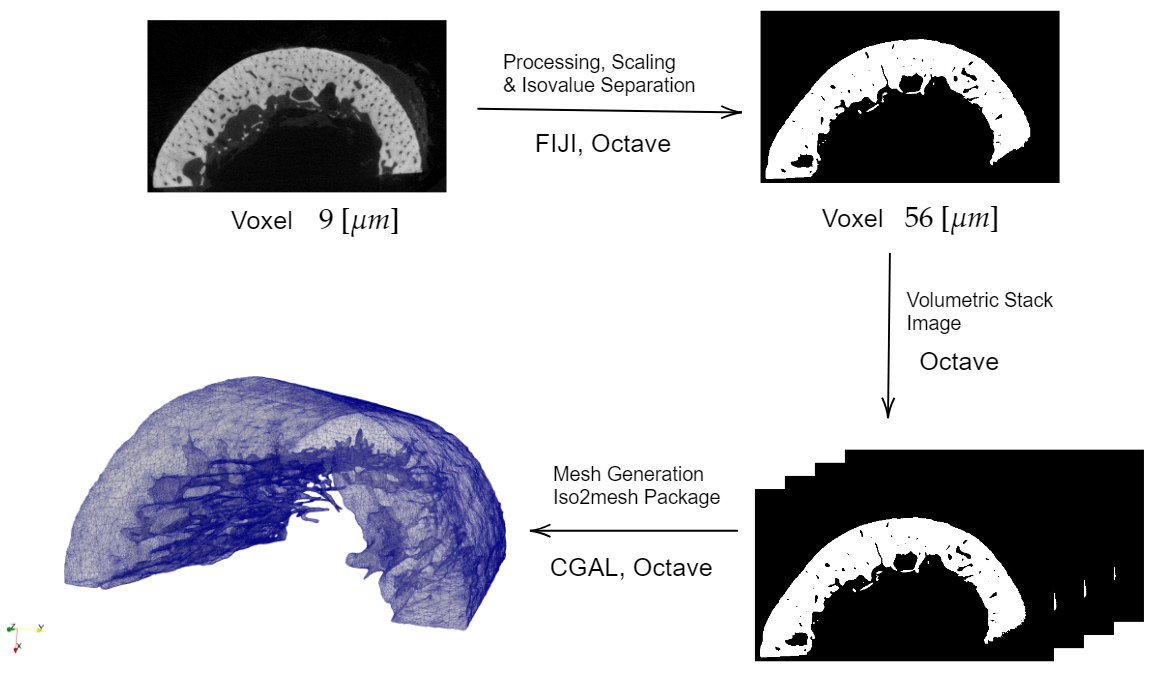
\includegraphics[scale=.5]{images/ImgExt/DiagramMeshGeneration.png}
	\caption{Pipeline: The mesh generation involves a sequence of different softwares that generates the desired domain where the simulations takes place.}
	\label{DiagramMeshGeneration}
\end{figure} 

The 3-dimensional elastodynamic study of the homogenized bone is done by considering the above mesh generation (\ref{DiagramMeshGeneration}) ignoring the labeled sets, thus defining and uniform interior mesh being adaptive to the surface irregularities.
To keep the scaled distance to the experimental setting, its used $1000$ slices from the stack, thus defining real $56 \, [mm]$ of cortical bone geometry.
The objective then is to recover the \textit{Lamb}-waves associated to the 2-dimensional model but now incorporating the surface effect from the curvature and irregularities, that are expected to affect the behavior of the \textit{Lamb}-curves and thus recorded signal itself.
By applying the generation procedure described before it follows the realistic irregular mesh pictured in (\ref{HomBoneMeshFile}). It characterizes a cortical bone sample of $56 \, [mm]$ length in the long direction describing a thickness of $\sim 1.8 [mm]$. 

\begin{figure}[!h]
	\centering
	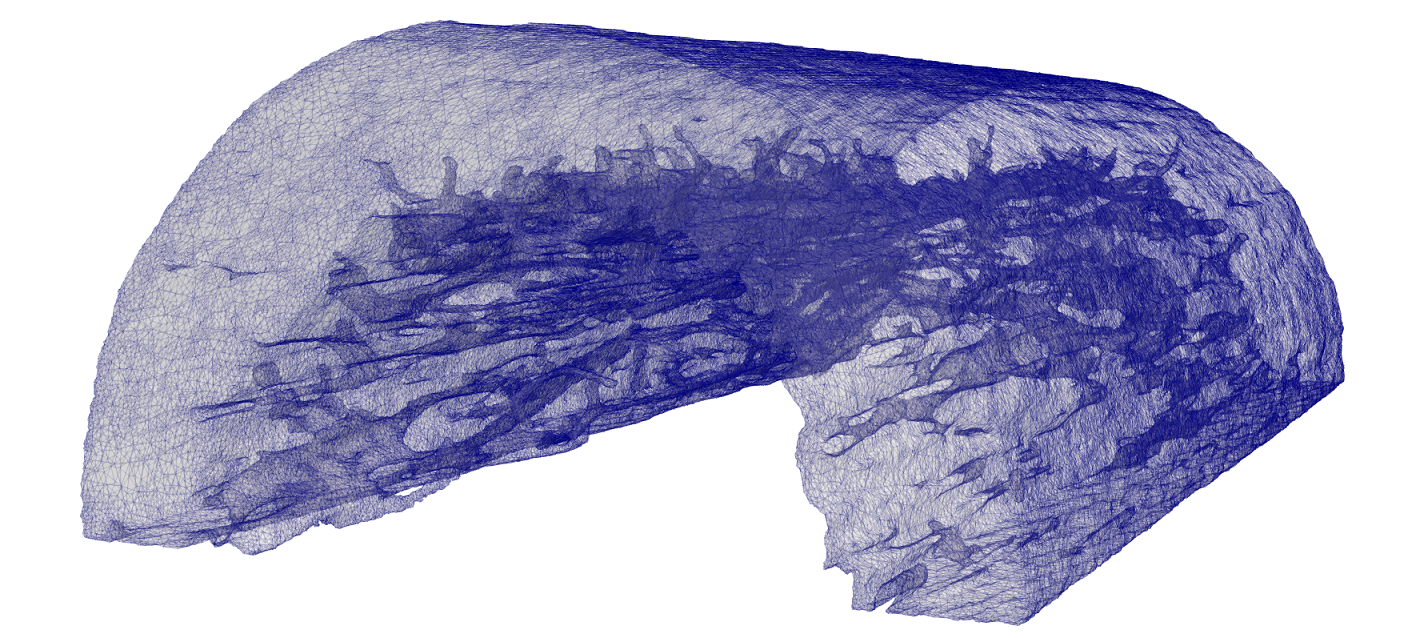
\includegraphics[width=0.8\textwidth]{images/ImgExt/CorticalBoneS1000OPT20-View.png}
	\caption{Mesh Generated from 1000 Slices from $\mu-CT$ images using the mesh-generation diagram (\ref{DiagramMeshGeneration}). It characterizes a cortical bone sample of $56 \, [mm]$ length in the long direction associated to a thickness $\sim 1.8 [mm]$ and experimentally tested porosity of $\sim 11 \%$. Explicitly, the mesh is described by $432,280$ vertices with $1,393,709$ tetrahedras.}
	\label{HomBoneMeshFile}
\end{figure} 

 \subsubsection{Simulation and Results}

The configuration is defined similar to the cylindrical case. The figure (\ref{HomBoneSubdomainsFile}) describes explicitly the settings of rectangular sources and receivers implemented, each one defined by a width of $\sim 0.8 [mm]$ with height $\sim 8 [mm]$ located at the top surface of the mesh. As in the cylinder case, the receivers record force-signal of type $\sigma^{hom}(u)\cdot n$ over each of the subdomain locations.
\begin{figure}[!h]
	\centering
	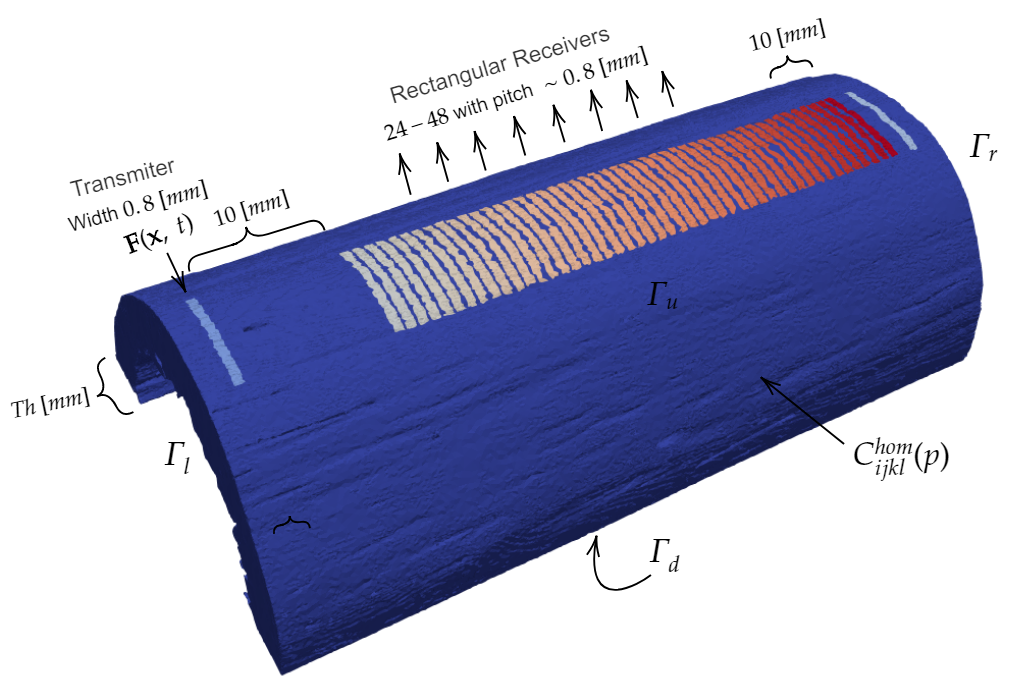
\includegraphics[width=0.8\textwidth]{images/ImgExt/Cortical3dsc04Mesh1000Fill-MeshBoundaries.png}
	\caption{The colors markers define the different subdomains associated to the mesh (\ref{HomBoneMeshFile}). It is described $48$ receivers and a transmitter locations in a array-like form resembling the experimental transducer. Moreover, each subdomain is defined approximately by $\sim 200$ marked tetrahedral cells.}
	\label{HomBoneSubdomainsFile}
\end{figure} 
The adaptive mesh (\ref{HomBoneMeshFile}) resembles a real geometry by meshing the irregularities on the inner surface characteristics of a natural cortical bone sample. Over such geometry is simulated an elastodynamic model propagating a guided wave and thus generating the guided-waves shown in (\ref{FK-HomBone-DiagramS1P11M18}) as shown in figure (\ref{HomBone-TimeStep}). Varying in color intensity, it is shown the wave-front interacting with the non-uniform mesh. Moreover, different view-planes show direct impact in the wave behavior as it interacts with the inner irregular surface, creating points of high displacement. This kind of behavior not observed on the cylindrical case studied before, thus becoming an inherent effect from the irregularities.

\begin{figure}[!h]
	\centering
	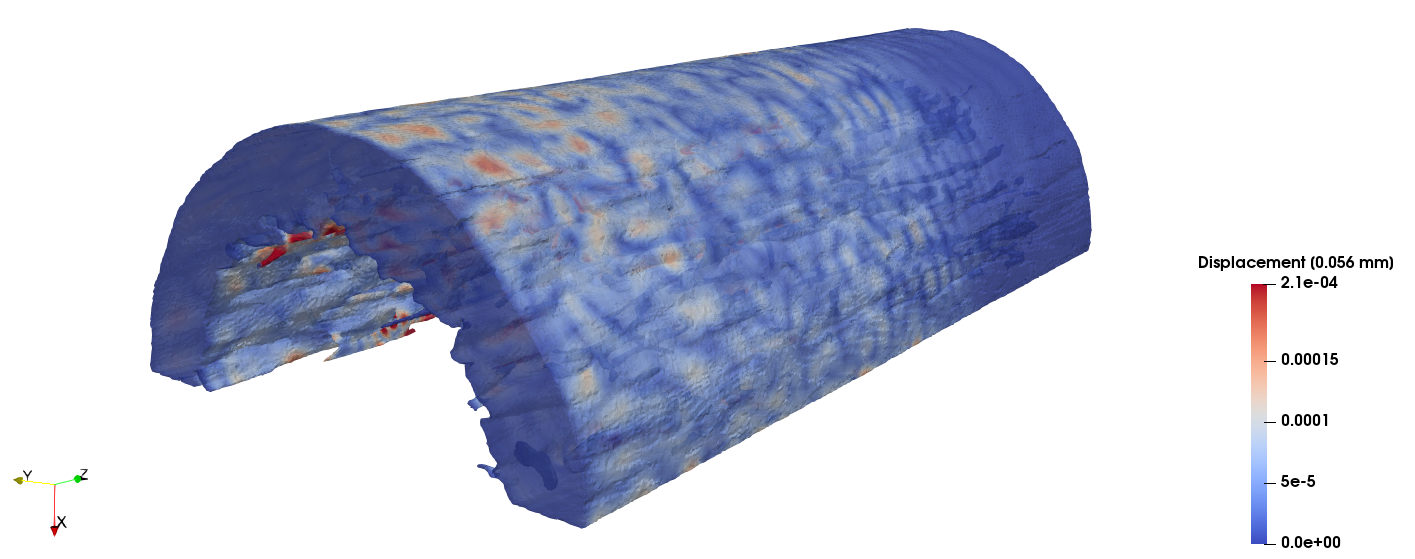
\includegraphics[width=0.8\textwidth]{images/ImgExt/Cortical3dsc04Mesh1000Fill-T80.png}
	\caption{The elastodynamic simulation over the irregular mesh is shown at instant $32 \, [\mu s]$, characterizing the wave-front propagation using a intensity color-scheme. The right-hand side bar contains the scale over the simulation, at $0.056 \, [mm]$ associated to the voxel size.}
	\label{HomBone-TimeStep}
\end{figure} 

\begin{rem}
The elastodynamic model simulated over this complex domain at $\sim 80 \, [\mu m]$ required 2 cores of a Xeon E5-2660 v2 processor with $\sim 8$ Gb of DDR3 RAM and $\sim 7$ days of computation time. It enables us to obtain complex wave-front propagation affected by the irregularities of the domain.
\end{rem}

The effect produced on the guided-wave from the interaction with the irregularities on the domain are shown in the $(f,k)$-diagram of figure (\ref{FK-HomBone-DiagramS1P11M18}). It shows a clear discrepancy between the reconstructed modes recorded at the receptors and the reference \textit{Lamb}-curves. The main variation is shown on the first anti-symmetric and symmetric modes, which does not fit within the expected behavior. Nevertheless, it can be seen that second modes have behavior fitting the references.  
\begin{figure}[!h]
	\centering
	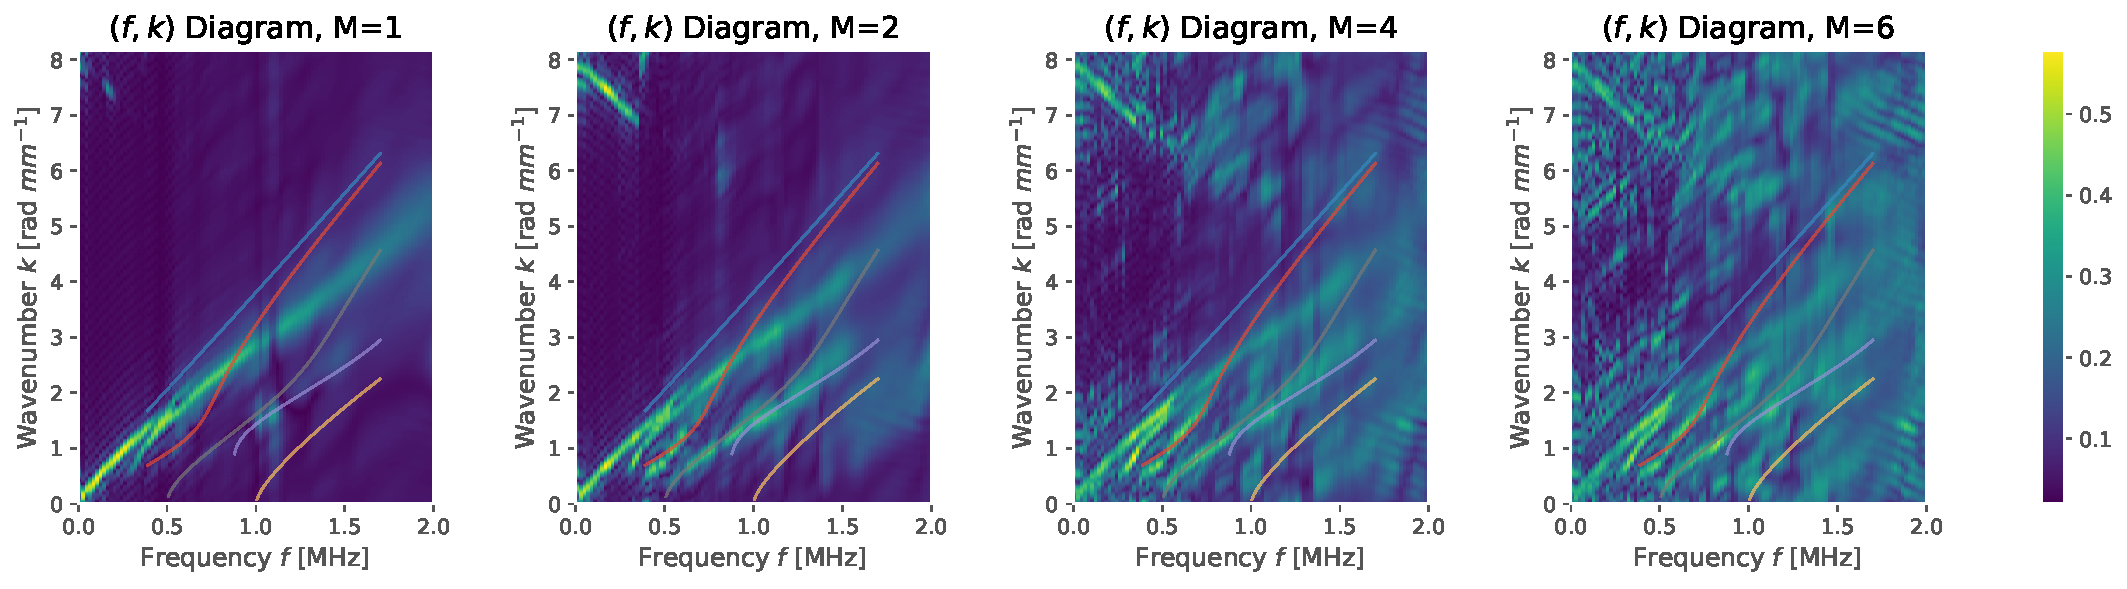
\includegraphics[width=\textwidth]{images/ClusterSim/3DCorticalS1000TimeP11TransIsoFKW18.pdf}
	\caption{Numerically simulated $(f,k)$-diagram of a 3-dimensional realistic-geometry. Setting of one-source with $11\%$ porosity and $\sim 1.8 [mm]$ thickness. The green lines defines \textit{Lamb} curves created from recording of the wave-guide being the others associated to a reference model.}
	\label{FK-HomBone-DiagramS1P11M18}
\end{figure} 

Similarly, singular values associated to data recording described by (\ref{FK-HomBone-DiagramS1P11M18}) are given on (\ref{SVD-HomBone-S1P11M18}) which resembles realistic values given the input force used. The figure shows the first three modes in realistic magnitude scale $(0, 20) \, [dB]$, being the rest of modes of lesser importance given the presence of noise in realistic measurements that should vanish the rest of modes.
\begin{figure}[!h]  
	\centering
	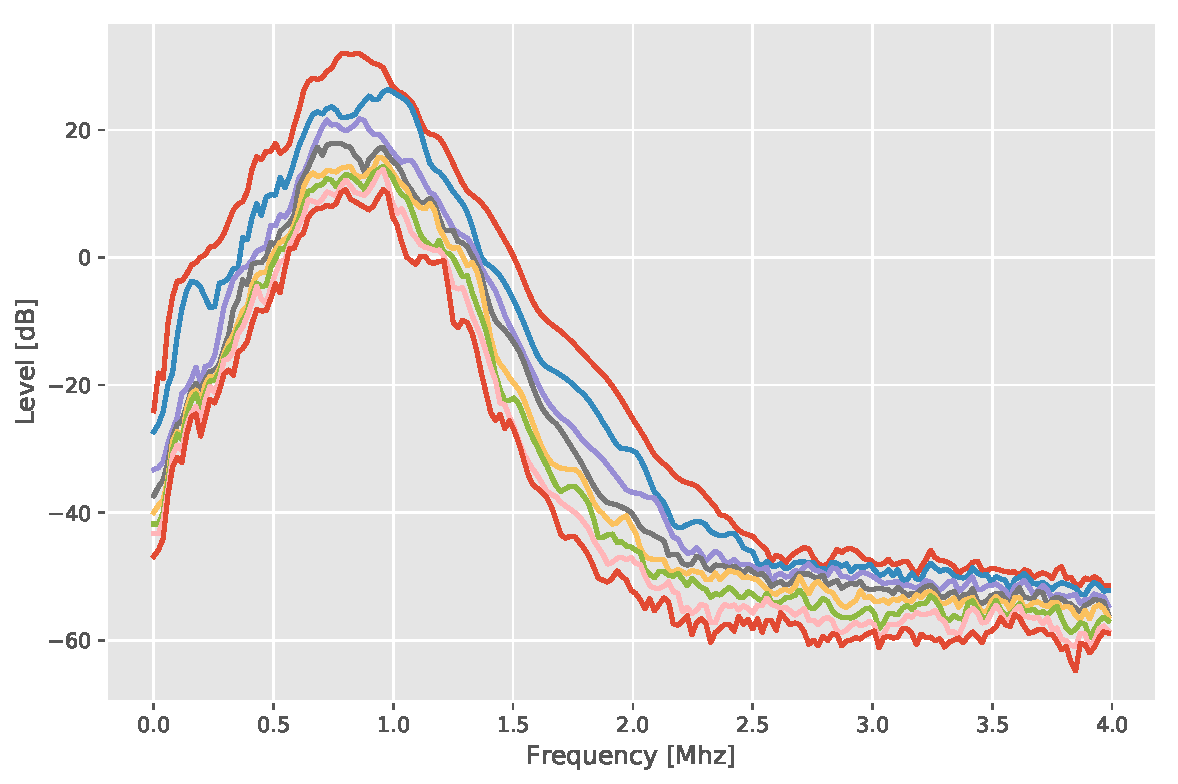
\includegraphics[scale=.5]{images/ClusterSim/3DCorticalS1000TimeP11TransIsoFKW18_SV.pdf}
	\caption{Singular values obtained by the SVD decomposition of the recorded signal from the simulation \ref{FK-Cyl-DiagramS1P11M18}}
	\label{SVD-HomBone-S1P11M18}
\end{figure}

In comparison with the half-cylinder case it's shown a clear variation on the general wavefront behavior, expressed in modes not align with respect to the reference cases for the parameters used in the simulation. Moreover, figure (\ref{FK-HomBone-DiagramS1P11M18}) shows clear signal distortion at the high frequency range of $(1, 2) [Mhz]$ for all the different \textit{Lamb}-curves involved, expressed in color diffusion within the curves. Explicitly, at higher $M$ values, which characterize the amount of receptors information to analyze, shows clear interaction within the domain mesh, thus more error fitting associated to the inverse problem solution.

On the other hand, figure (\ref{FK-Cyl-DiagramS1P11M18}) associated to the half-cylinder setting describes a more regular behavior of the curves in all the frequency range, corresponding to a wave-front in which the curvature effect does not affect the main axial propagation, thus describing at each $M$ values clear \textit{Lamb}-curves, thus fully comparative signal with the 2-dimensional case. The explanation to such behavior relates to missing interaction within the inner irregularities that fully deform the characteristic wave propagation.


%\subsubsection{Fully Porous Material}
%The save Pipeline (\ref{DiagramMeshGeneration}) is used for the mesh generation, now without homogenized coefficients and therefore taking into account the variation on the elastic coefficients depending on the presence of mesoscale structure and cavities.
